\begin{frame}
\frametitle{About This Work...}

\emph{Cleaning Trajectory Data of RFID-monitored Objects through Conditioning under Integrity}~\cite{DBLP:conf/edbt/FazzingaFFP14}\\
B.~Fazzinga, S.~Flesca, F.~Furfaro, F.~Parisi.\\~\\

% \emph{Handling False Negatives in Indoor RFID Data}.~\cite{baba2014handling} \\
% A.I.~Baba, H.~Lu, T.B.~Pedersen, X.~Xie\\~\\

\begin{itemize}
  \item Published at \emph{EDBT' 2014}. %, \emph{MDM' 2014}.
  \item A probabilistic framework is introduced for reducing the inherent uncertainty of trajectory data collected for RFID-monitored objects.
  \item The framework cleans trajectories by conditioning them to the event that integrity constraints encoding some knowledge about the map and the motility characteristics of the monitored objects hold.
\end{itemize}

\end{frame}

%------------------------------------------------

\begin{frame}
\frametitle{Motivation}

\begin{itemize}
  \item Pervasive use of RFID devices as a support for object tracking
  \begin{fitemize}
    \item monitoring of people, animals and objects inside museums, shools, hospital etc.
    \item context-aware information.
  \end{fitemize}
  \item There exists ambiguity in the raw RFID data.
  \begin{fitemize}
    \item no one-to-one correspondence between locations and readers, no way to deterministically decide the location given that a set of readers detected an object.
    \item the same location may constain different reader's detection zones, the same reader may detect different objects at different locations, also false negatives.
  \end{fitemize}
\end{itemize}

\end{frame}

%------------------------------------------------

\begin{frame}
\frametitle{Ambiguity of RFID Data}

\begin{columns}

  \column{0.4\textwidth}
  \begin{figure}[tb]
    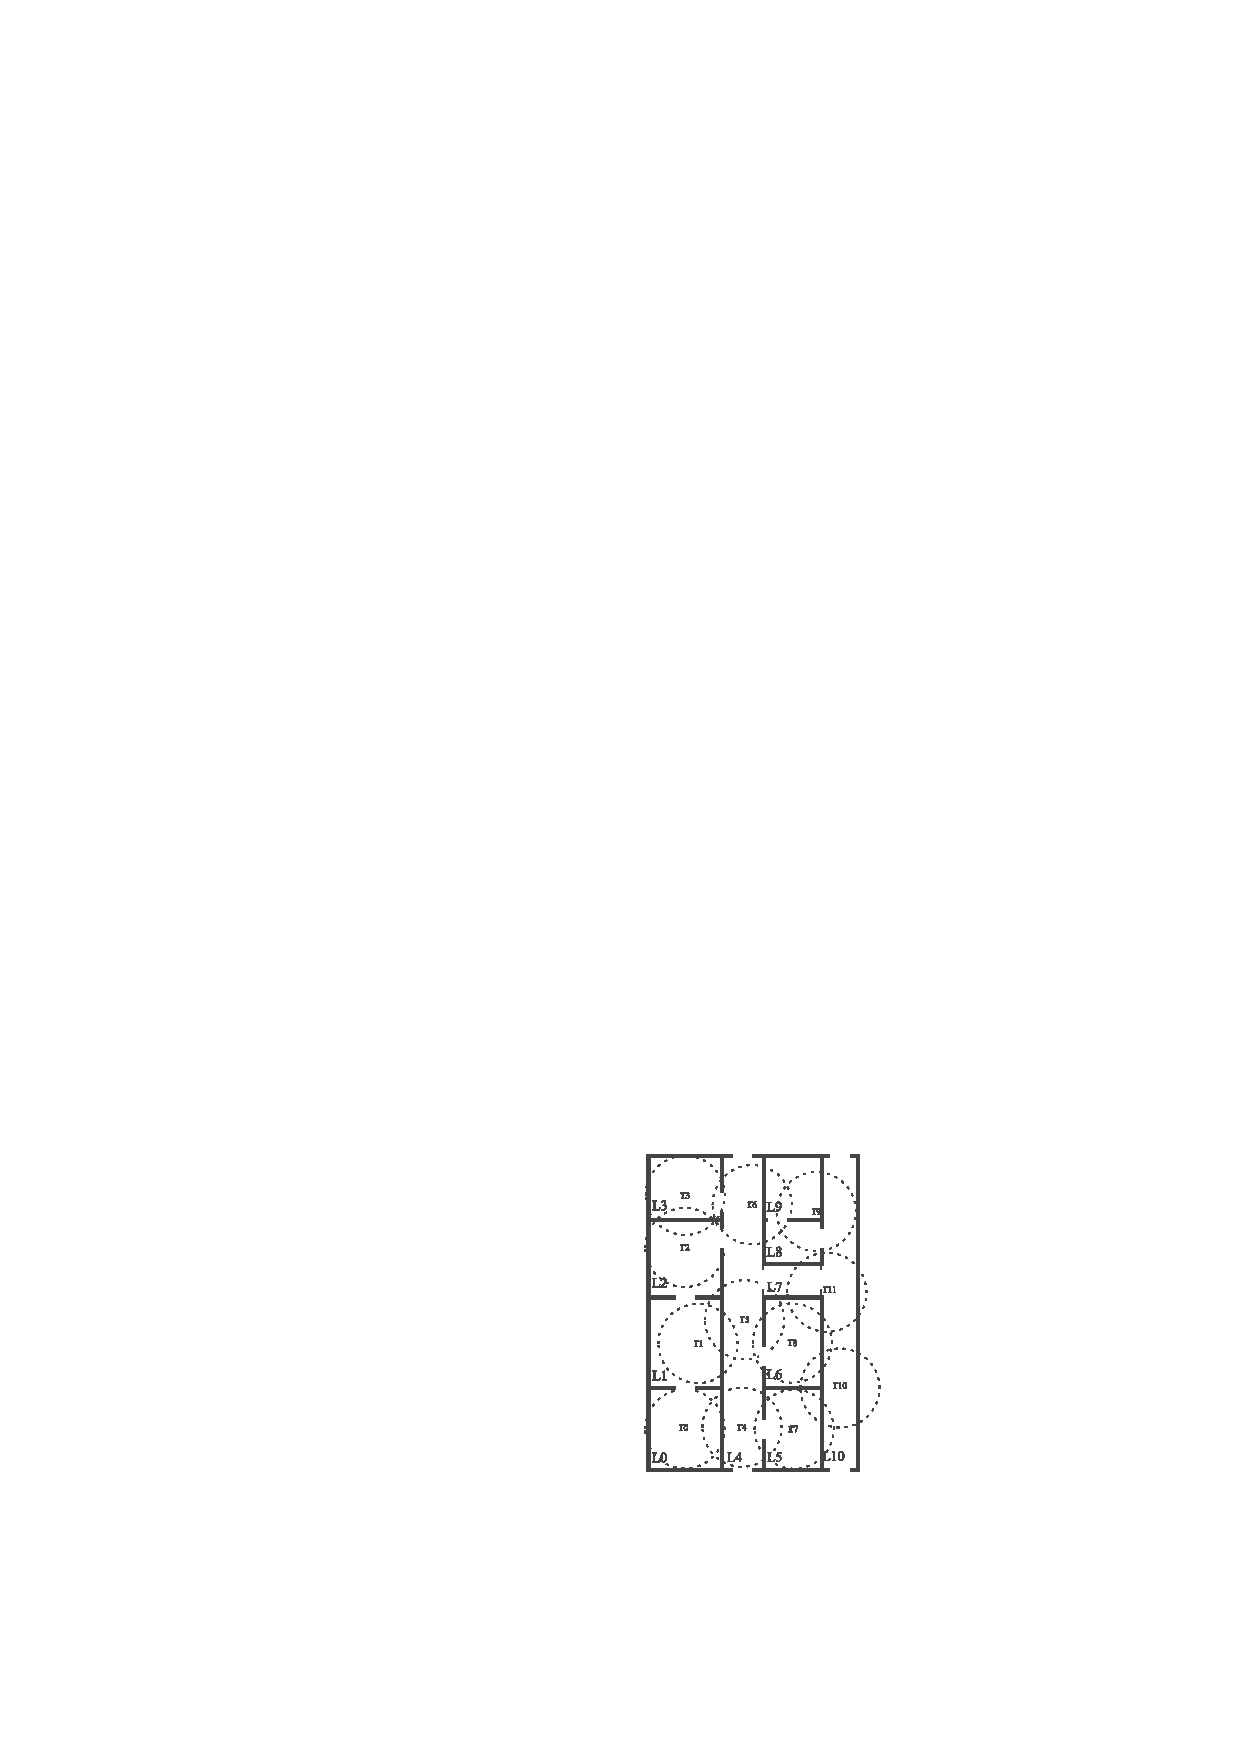
\includegraphics[width=\columnwidth]{figures/3-4/3-4-1.pdf}
  \end{figure}

  \column{0.6\textwidth}
  \begin{example}
    \fsize{
    an object $o$ was detected at some instant by both reader $r_1$ and $r_5$, two locations are possible, $L_1$ and $L_4$. Analogously, if $o$ was detected by $r_3$ only, we cannot conclude that it was surely in $L_3$, as it could be the case that $r_2$ failed to detect it despite it was close enough to its antenna.
    }
  \end{example}

  \ssize{\textrm{\\this suggests that the association readers/locations can be naturally modeled in probabilistic terms. For instance by a probability distribution $p^a(l|R)$ defined for each location $l$ and set $R$ of readers.}}
  $p^a(L_1|\{r_1, r_5\}) = p^a(L_4|\{r_1, r_5\}) = 0.5$
  $p^a(L_0|\{r_0\}) = 1$

\end{columns}

\end{frame}

%------------------------------------------------

\begin{frame}
\frametitle{Ambiguity of RFID Data}

\begin{columns}

  \column{0.4\textwidth}
  \begin{figure}[tb]
    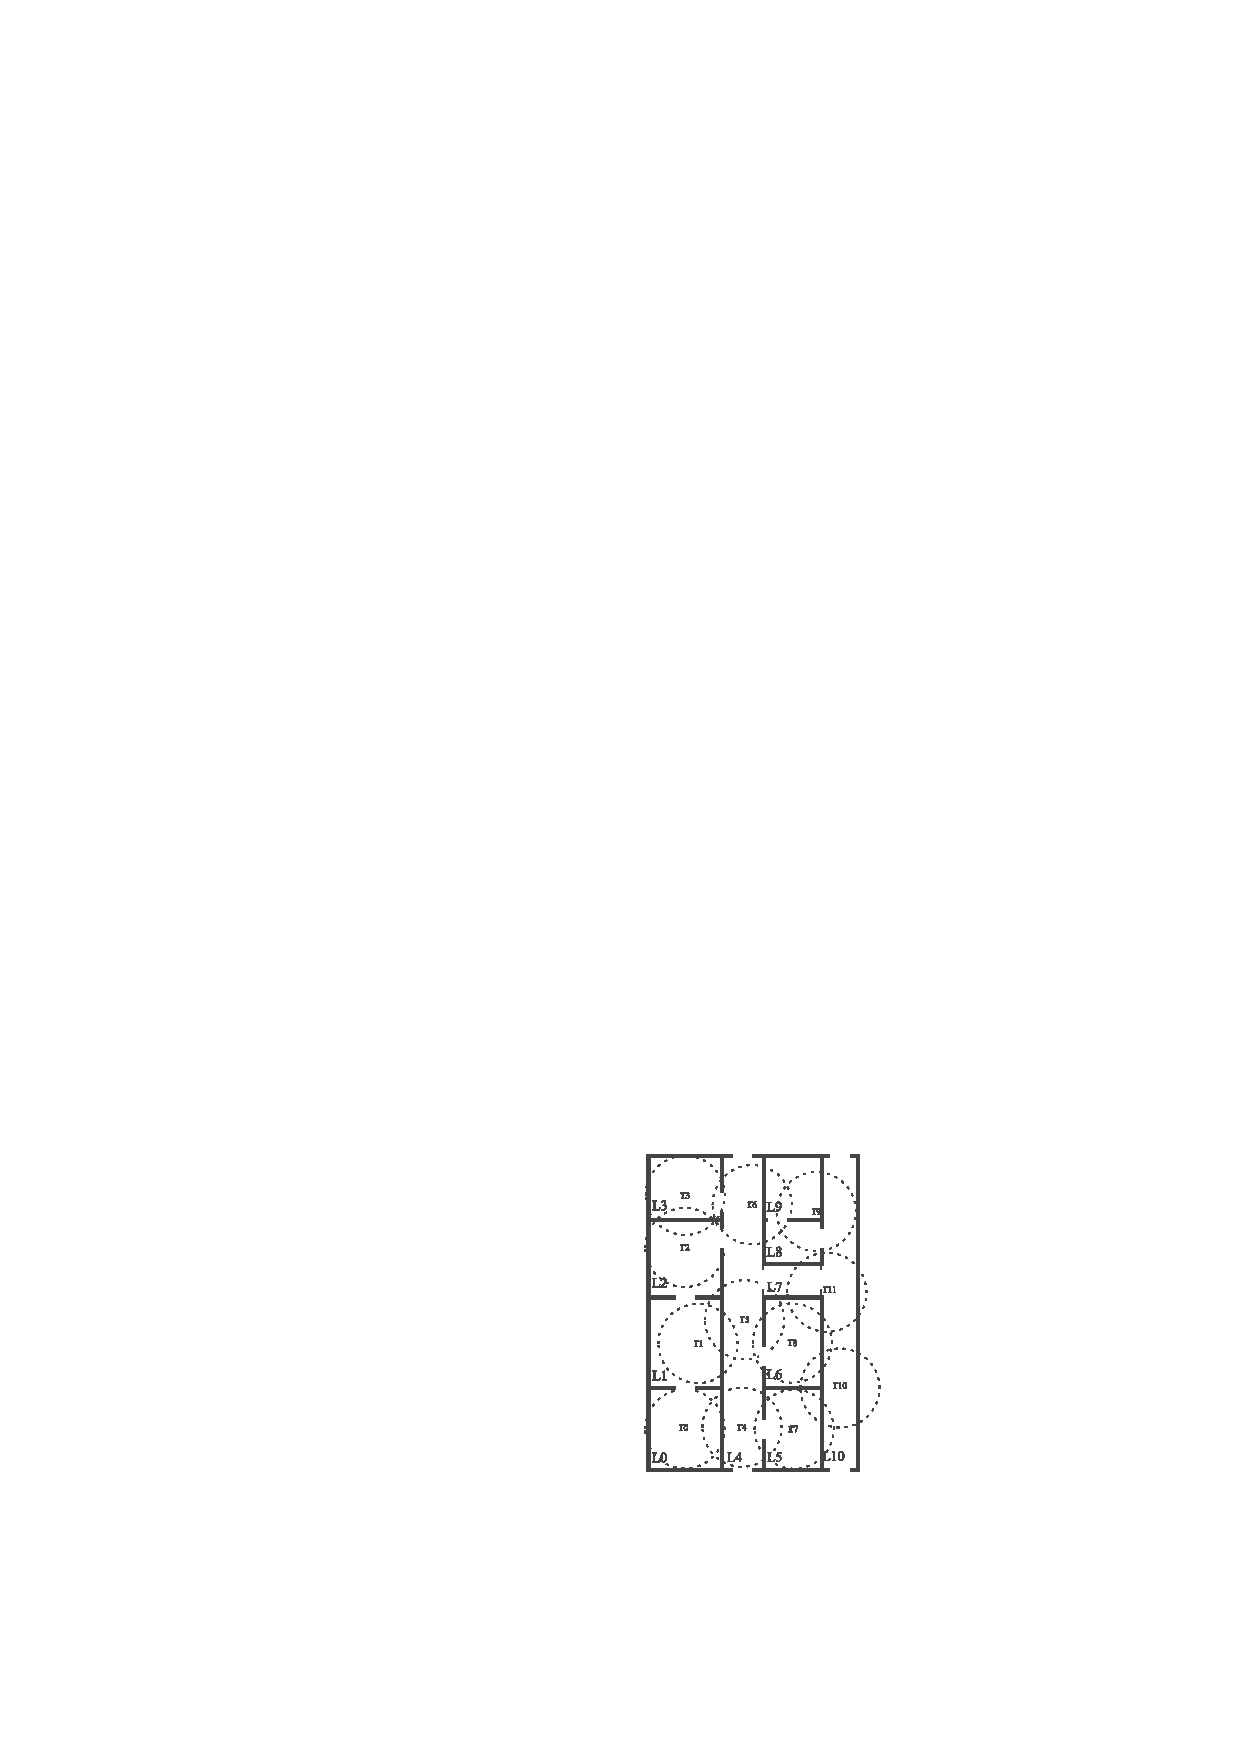
\includegraphics[width=\columnwidth]{figures/3-4/3-4-1.pdf}
  \end{figure}

  \column{0.6\textwidth}
  \ssize{\textrm{things become more complex when trying to translate a sequence of readings into possible trajectories, a naive way is to consider the steps of the trajectory independent from each other.}}

  \begin{example}
    \ssize{
    assume that at instants(timestamps) 0 and 1, $o$ is detected by both $r_1$ and $r_5$, while at instant 2 it's detected by $r_0$. Assume that $p^a(l|R)$ is used, i.e., objects detected by $r_1$ and $r_5$ are at location $L_1$ with probability 0.5 and at $L_4$ with probability 0.5, detected by $r_0$ are at $L_0$ with probability 1. Reasoning only on the basis of these probabilities and exploiting no further knowledge, the trajectories followed by $o$ can be: $t_1: L_1L_1L_0$, $t_2: L_1L_4L_0$, $t_3: L_4L_1L_0$, $t_4: L_4L_4L_0$, each with pribability 0.25.
    }
  \end{example}

\end{columns}

\end{frame}

%------------------------------------------------

\begin{frame}
\frametitle{Ambiguity of RFID Data}

The independence assumption allows for reasoning about tracjectory probabilities as follows.\\~\\
\pause

Consider an object $o$ moving over time interval $\mathcal{T} = [\tau_1,...,\tau_n]$, and the sequence of readings $\Theta = \langle \tau_1, R_1 \rangle, ..., \langle \tau_n, R_n \rangle$, meaning that at each $\tau_i \in \mathcal{T}$, $o$ was detected by the set $R_i$ of readers.\\~\\
\pause

The probability that $o$ followed the trajectory $t = l_1, ..., l_n$ can be expressed (under the independence assumption) as $p^a(t|\Theta) = \prod_{i=1}^n p^a(l_i|R_i)$.\\~\\
\pause

Unfortunately, the probabilities returned by $p^a(t|\Theta)$ can be very different from those returned by the ``actual'' probability distribution $Pr(t|\Theta)$ as the following example.

\end{frame}

%------------------------------------------------

\begin{frame}
\frametitle{Ambiguity of RFID Data}

\begin{columns}

  \column{0.4\textwidth}
  \begin{figure}[tb]
    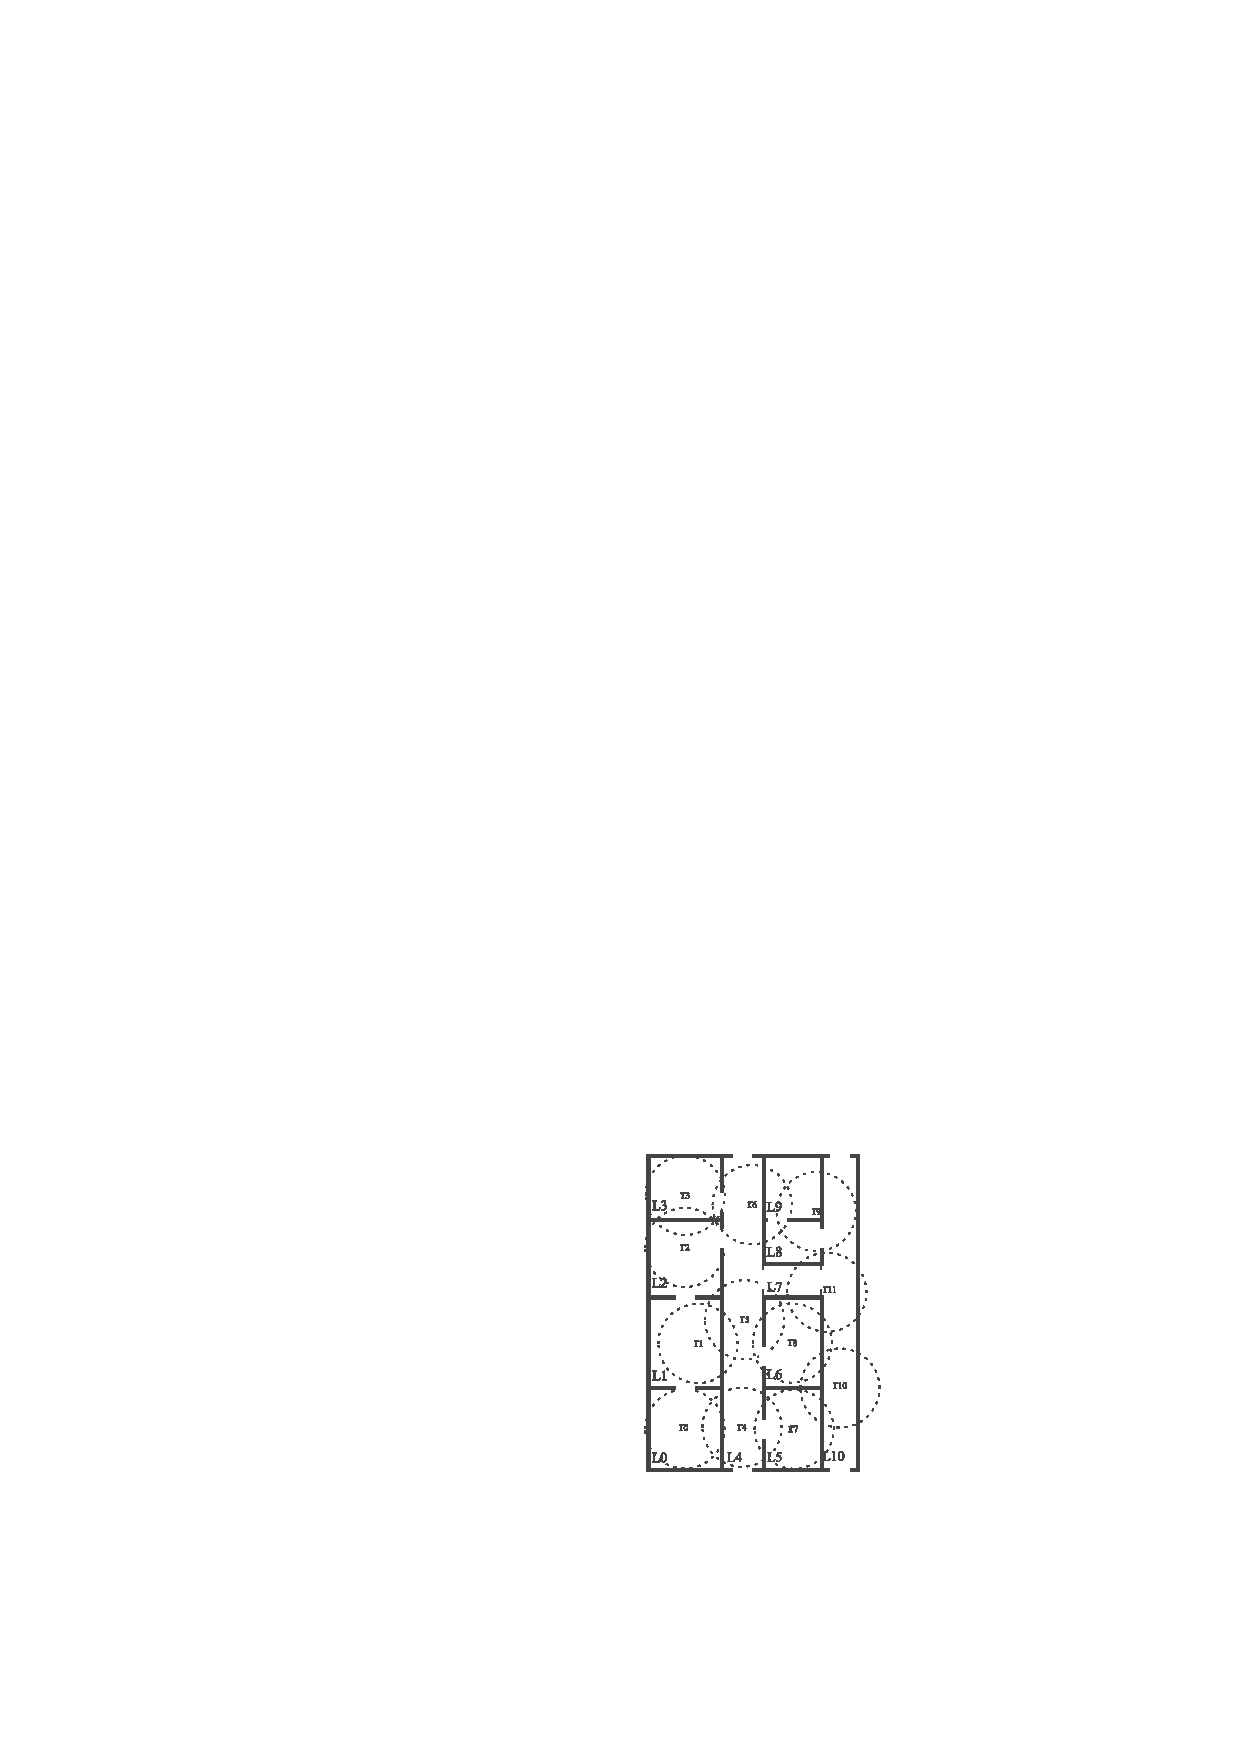
\includegraphics[width=\columnwidth]{figures/3-4/3-4-1.pdf}
  \end{figure}

  \column{0.6\textwidth}

  \begin{example}
    \ssize{
    For the four possible trajectories $t_1: L_1L_1L_0$, $t_2: L_1L_4L_0$, $t_3: L_4L_1L_0$, $t_4: L_4L_4L_0$, we can infer only $t_1$ is the only correct interpretation of the data according to the map. Since $L_0$ and $L_4$ have no direct connection, and $L_1$ is directly connected to $L_0$ by not to $L_4$. Thus a correct probability distribution over the possible trajectories is at follows: $Pr(t_1|\Theta) = 1$, $Pr(t_2|\Theta) = Pr(t_3|\Theta) = Pr(t_4|\Theta) = 0$, where $\Theta = \theta_1, \theta_2$, and $\theta_1 = \langle \tau_1, \{ r_1, r_5 \} \rangle $, $\theta_2 = \langle \tau_2, \{ r_0 \} \rangle $.
    }
  \end{example}

  \ssize{\textrm{the point is that even $p^a(l|R)$(also $p^a(t|\Theta)$) is easy to obtain, finding a formulation for $Pr(t|\Theta)$ is very hard, as it requires analyzing and encoding the correlations among possible positions over time.}}

\end{columns}

\end{frame}

%------------------------------------------------

\begin{frame}
\frametitle{Target of This Work}

\begin{problem}
  given a sequence of readings $\Theta$ and exploiting the knowledge of $p^a(l|R)$ (and thus $p^a(t|\Theta)$), how can we effectively and efficiently revise $p^a(t|\Theta)$ so that it takes into account possible correlations inside the data, thus obtaining a better estimate of $Pr(t|\Theta)$.
\end{problem}

Intuitively enough, revising $p^a(t|\Theta)$ according to the known correlations can be viewed as a cleansing problem: the data to be cleaned are the (probabilistic) trajectories resulting from using $p^a(t|\Theta)$ to interpret the sequence of readings, and the cleansing task consists in revising the probablitisties assigned to these trajectories.

\end{frame}

%------------------------------------------------

\begin{frame}
\frametitle{Cleansing RFID Data}

Exploiting the knowledge on the map and on the motility characteristics:\\~\\

\conceptbf{Direct-unreachability Constraint} can be naturally derived on the connectivity between pairs of locations.\\~\\

\conceptbf{Traveling-time Constraint} can be derived on the time needed for reaching a location starting from another one.

\end{frame}

%------------------------------------------------

\begin{frame}
\frametitle{Cleansing RFID Data}

\begin{columns}

  \column{0.4\textwidth}
  \begin{figure}[tb]
    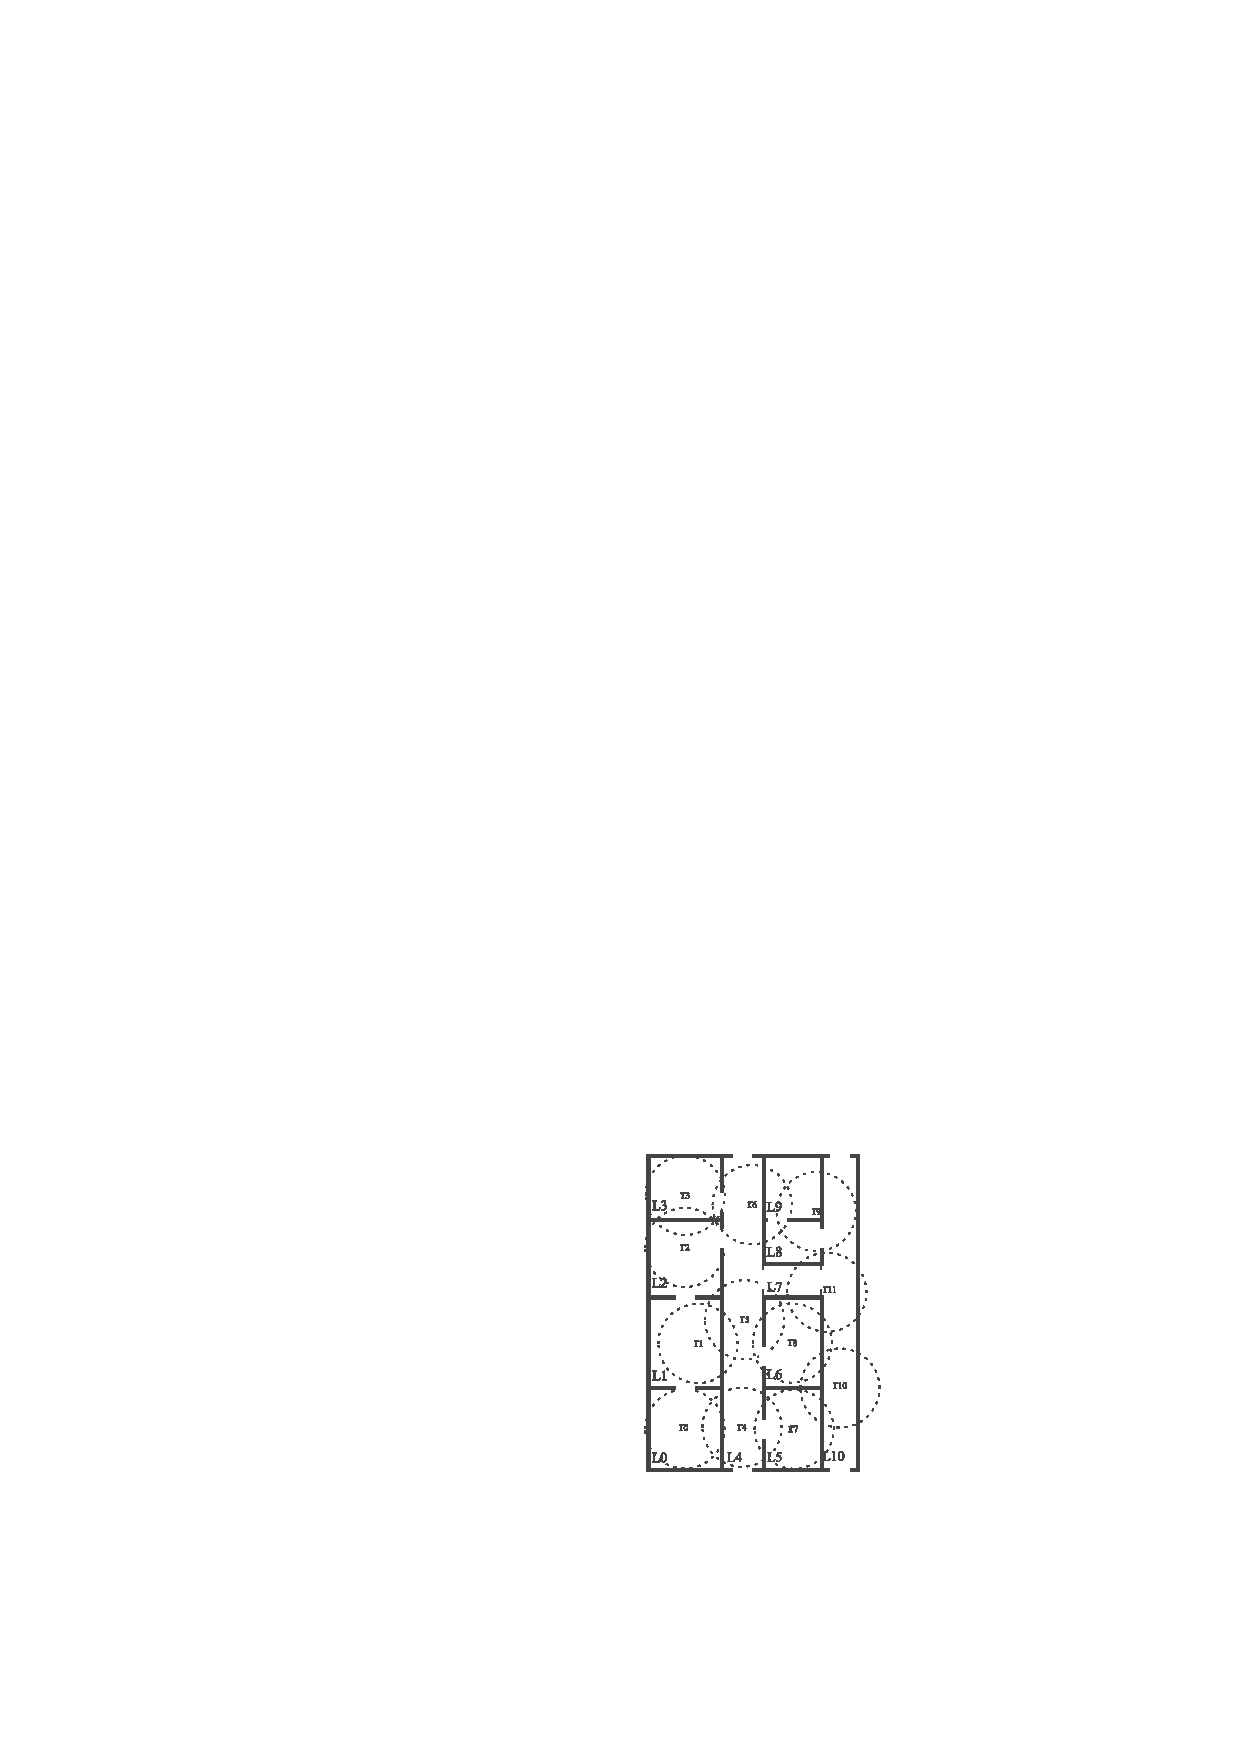
\includegraphics[width=\columnwidth]{figures/3-4/3-4-1.pdf}
  \end{figure}

  \column{0.6\textwidth}

  \begin{example}
    \ssize{
      the map easily implies a set of direct-unreachability constraints, one for each pair of rooms which are not directly connected through a door, such as $L_0,L_4$ and $L_1,L_4$.\\
      The map implies further constraints, other than direct unreachability. E.g., it says that $L_0$ and $L_5$, althrough close to one another, are connected only by a pretty long path. Reasonably, it can be imposed that $15 sec$ are required to go through this path. (called ``traveling-time constraint'').
    }
  \end{example}
  \ssize{\textrm{the above example explains how considering integrity constraints can reduce uncertainty, as it allows trajectories to be removed from the valid interpretations of data.}}

\end{columns}

\end{frame}

%------------------------------------------------

\begin{frame}
\frametitle{Cleansing RFID Data}

\fsize{

\conceptbf{The target of this work} becomes how to reasonably combine the integrity constraints with the \emph{a-priori} probabilistic model encoded by $p^a(l|R)$, in order to devise a mechanism for revising the a-priori probabilities of the remaining valid trajectories and making them sum up to 1.\\~\\

A rigorous approach~\cite{koch2008conditioning,flesca2014consistency} is to perform \conceptbf{conditioning}: starting from the a-priori probabilities(without constraints), the probabilities of the trajectories are re-evaluated as conditioned to the event that the constraints are satisfied.\\~\\

That is, given a set $\mathcal{IC}$ constraints, probabilities of the form $p^a(t|\Theta)$ are revised into $p^a(t|\Theta \wedge \mathcal{IC})$. This way, the probability of invalid trajectories becomes 0, while that of each valid trajectory becomes the ratio of its a-priori probability to the overall a-priori probability of the valid trajectories.

}

\end{frame}

%------------------------------------------------

\begin{frame}
\frametitle{Preliminaries}

\ssize{
\begin{table}
    \begin{center}
    \begin{tabular}{|c|c|}
    \hline
        \textbf{Notation} &   \textbf{Meaning}                    \\
    \hline
        $o$      &   a single object equipped with RFID tag        \\
    \hline
        $\mathcal{R} = \{ r_1, ..., r_k \}$      &   a set of RFID readers     \\
    \hline
        $\mathcal{L} = \{ l_1, ..., l_n \}$      &  the set of locations       \\
    \hline
        $\mathcal{T} = [0..\tau_f]$      &  the time interval over monitoring       \\
    \hline
        $\theta = \langle \tau, R \rangle$      &  a reading of $o$ \\
    \hline
        $\Theta$        &   a set of readings, a \emph{reading sequence} (r-sequence) \\
    \hline
        $p^a(l|R)$        &   the \emph{a-priori} probability  \\
    \hline
        $X_{\theta}$        &   the discrete random variable \\
    \hline
        $f(X_{\theta} = l) = p^a(l|\theta[readers])$        &   probability density funtion for the random variable \\
    \hline
    \end{tabular}
    \end{center}
\end{table}
}

\end{frame}

%------------------------------------------------

\begin{frame}
\frametitle{Preliminaries}

\begin{definition}[probabilistic location sequence (l-sequence)]
  given $p^a(l|R)$ and an r-sequence $\Theta$, we define the \emph{probabilistic location sequence} corresponding to $\Theta$ (according to $p^a(l|R)$) as the set $\Gamma = \{ X_{\theta} | \theta \in \Theta \}$.
\end{definition}

\fsize{
The l-sequence $\Gamma$ corresponding to the r-sequence $\Theta$ for $o$ over $\mathcal{T}$ will be denoted as a pair $\Gamma = \langle \Lambda,p \rangle$.
\begin{itemize}
  \item $\Lambda$ is a set of pairs of the form $\Lambda = \langle \tau, l \rangle$, with $\tau \in \mathcal{T}$ and $l \in \mathcal{L}$, containing at least one pair $\langle \tau, l \rangle$ for each $\tau \in \mathcal{T}$.
  \item $p$ assigns to each pair $\langle \tau, l \rangle \in \Lambda$ the value $f(X_{\theta} = l)$, where $\theta$ is the reading at time $\tau$, i.e., $p$ assigns to $\langle \tau, l \rangle$ the probability that the object was at location $l$ at time $\tau$, as implied by the PDF of the random variable.
\end{itemize}
}

\end{frame}

%------------------------------------------------

\begin{frame}
\frametitle{Preliminaries}

\begin{columns}

  \column{0.4\textwidth}
  \begin{figure}[tb]
    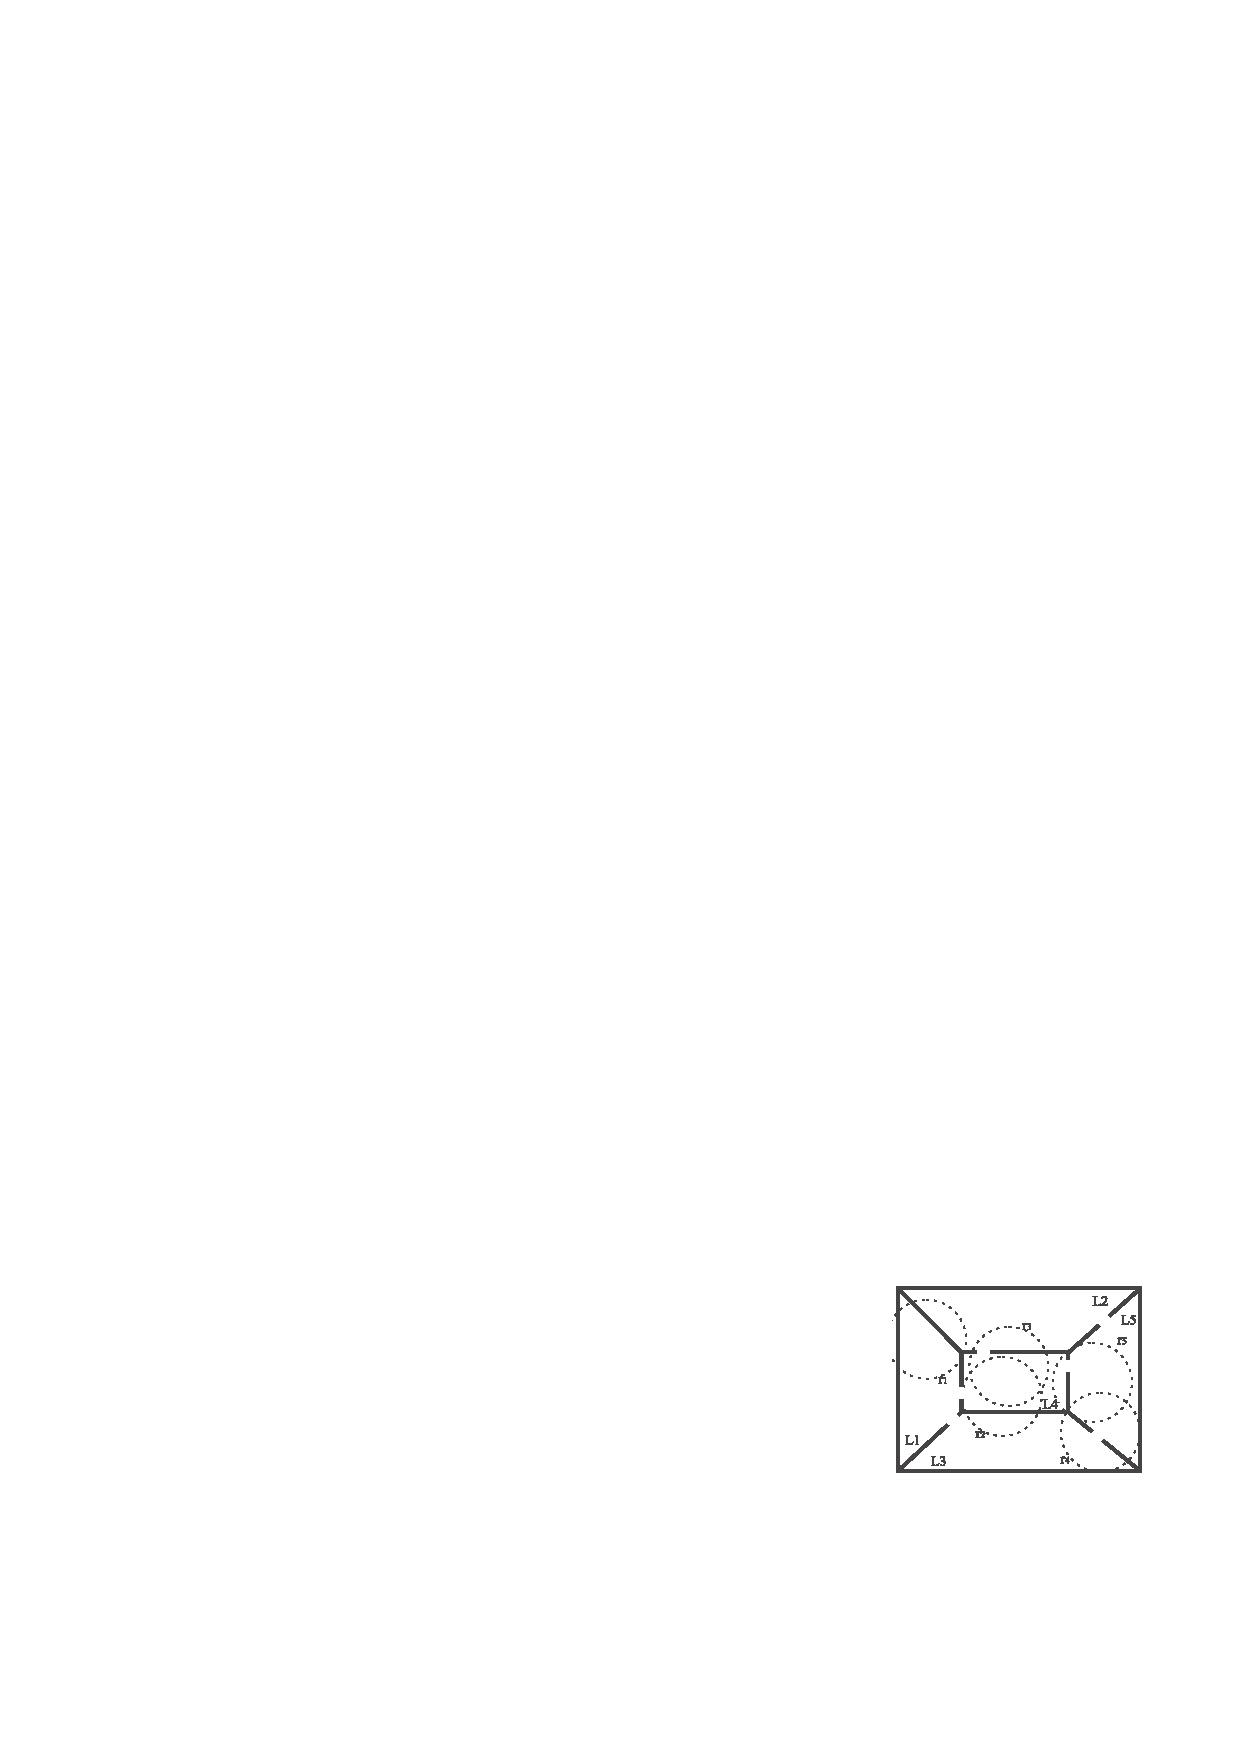
\includegraphics[width=\columnwidth]{figures/3-4/3-4-2.pdf}
  \end{figure}

  \column{0.6\textwidth}

  \begin{example}
    \ssize{
      consider the r-sequence $\Theta = \{ \langle 0, \{ r_1 \} \rangle, \langle 1, \{ r_2 \} \rangle, \langle 2, \{ r_4 \} \rangle \}$ and $p^a(l|R)$ s.t. $p^a(L_1|\{r_1\}) = \frac{6}{10}$, $p^a(L_2|\{r_1\}) = \frac{4}{10}$, $p^a(L_3|\{r_2\}) = \frac{1}{3}$, $p^a(L_4|\{r_2\}) = \frac{2}{3}$, $p^a(L_3|\{r_4\}) = \frac{2}{3}$, $p^a(L_5|\{r_4\}) = \frac{1}{3}$. The corresponding l-sequence $ \Gamma = \langle \Lambda, p \rangle $ is s.t. $ \Lambda = \{ \lambda_1 = \langle 0, L_1 \rangle, \lambda_2 = \langle 0, L_2 \rangle, \lambda_3 = \langle 1, L_3 \rangle, \lambda_4 = \langle 1, L_4 \rangle, \lambda_5 = \langle 2, L_3 \rangle, \lambda_6 = \langle 2, L_5 \rangle \} $, and $p(\lambda_1) = \frac{6}{10}$, $p(\lambda_2) = \frac{4}{10}$, $p(\lambda_3) = \frac{1}{3}$, $p(\lambda_4) = \frac{2}{3}$, $p(\lambda_5) = \frac{2}{3}$, $p(\lambda_6) = \frac{1}{3}$.
    }
  \end{example}

\end{columns}

\end{frame}

%------------------------------------------------

\begin{frame}
\frametitle{Preliminaries}

given a pair $\lambda = \langle \tau, l \rangle \in \Lambda$, denote the first and the second component of $\lambda$ with $\lambda[time]$ and $\lambda[loc]$ respectively.

\begin{definition}[Trajectory]
  Let $\Theta$ be an r-sequence over $\mathcal{T}$ and $\Gamma = \langle \Lambda,p \rangle$ be the l-sequence corresponding to $\Theta$. A trajectory over $\Gamma$ is a set $t \subseteq \Lambda$ of pairs such that, for each $\tau \in \mathcal{T}$, there is a unique pair $\lambda \in t$ such that $\lambda[time] = \tau$. The (a-priori) probablitity of $t$ is $p^a(t|\Theta) = \prod_{\lambda \in t}p(\lambda)$. For simplicity, we write $p^a(t|\Theta)$ as $p^a(t)$.
\end{definition}

The set of the trajectories over an l-sequence $\Gamma$ is denoted as $T(\Gamma)$. Given a trajectory $t$, the pair $\lambda \in t$ such that $\lambda[time] = \tau$ is said to be the $\tau$-th \emph{step} of $t$.

\end{frame}

%------------------------------------------------

\begin{frame}
\frametitle{Preliminaries}

\begin{columns}

  \column{0.4\textwidth}
  \begin{figure}[tb]
    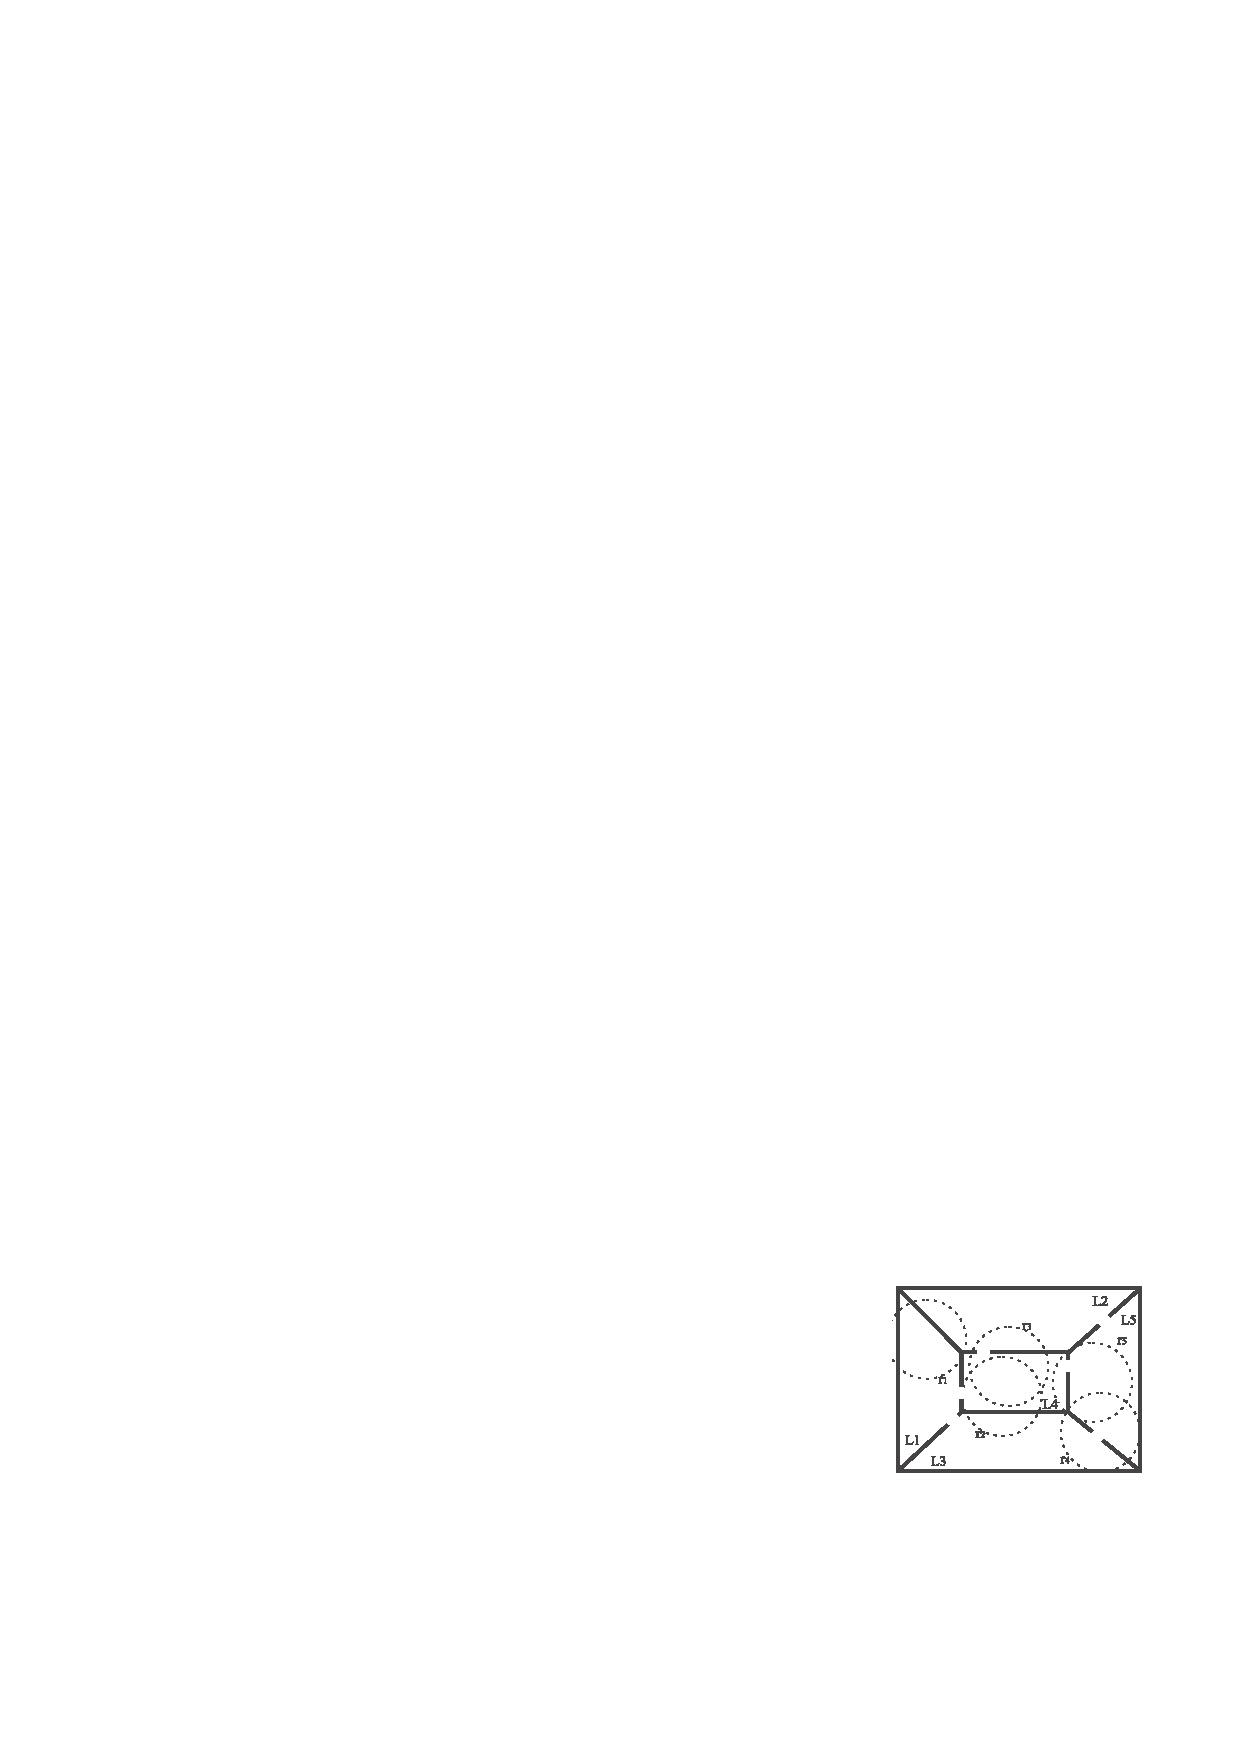
\includegraphics[width=\columnwidth]{figures/3-4/3-4-2.pdf}
  \end{figure}

  \column{0.6\textwidth}

  \begin{example}
    \ssize{
      2 out of the 8 trajectories over the l-sequence $\mathcal{T} = \langle \Lambda,p \rangle$ are $t_1 = \{\lambda_1, \lambda_3, \lambda_5\}$, which means that object $o$ went from $L_1$ to $L_3$ and stayed in $L_3$ for two consecutive timestamps, and $t_2 = \{\lambda_1, \lambda_3, \lambda_6\}$, which describes the case that object $o$ went from $L_1$ to $L_5$ through $L_3$. Their a-priori probabilities are $p^a(t_1) = p(\lambda_1) \cdot p(\lambda_3) \cdot p(\lambda_5) = \frac{12}{90}$, and $p^a(t_2) = p(\lambda_1) \cdot p(\lambda_3) \cdot p(\lambda_6) = \frac{6}{90}$.

    }
  \end{example}

\end{columns}

\end{frame}

%------------------------------------------------

\begin{frame}[allowframebreaks]
\frametitle{Constraints}

\begin{definition}[Direct Unreachability (DU) Constraint]
  Given two locations $l_1, l_2 \in \mathcal{L}$, a \emph{direct unreachability} constraint has the form $unreachable(l_1,l_2)$ and states that no object can reach $l_2$ from $_1$ in one time point.
\end{definition}

\begin{definition}[Traveling Time (TT) Constraint]
  Given two locations $l_1, l_2 \in \mathcal{L}$ and a non-negative integer $\nu$, a \emph{traveling time} constraint is of the form $travelingTime(l_1, l_2, \nu)$ and states that, for any object, the time needed to move from $l_1$ to $l_2$ is not less that $\nu$.
\end{definition}

\begin{definition}[Latency (LT) Constraint]
  Given a location $l \in \mathcal{L}$ and a non-negative integer $\delta$, a \emph{latency constraint} associated with $l$ is denoted as $latency(l,\delta)$ and imposes that every time an object goes into location $l$, it must stay in $l$ for at least $\delta$ time points.
\end{definition}

\vspace{15pt}
\fsize{\textrm{$DU$ constraints are implied by the structure of the map, and $TT$ constraints are implied by the minimum distances between the locations and the maximum speed of the objects. As regards latenct constraints, they take into account the physical inertia of objects, as well as the processing times (for doing some job).}}

\end{frame}

%------------------------------------------------

\begin{frame}
\frametitle{Integrity Constraints}

\begin{definition}[Integrity Constraints]
  Let $\Gamma = \langle \Lambda, p \rangle$ be an l-sequence and $\mathcal{IC}$ a set of \emph{integrity constraints}. A trajectory $t$ over $\Gamma$ is valid w.r.t $\mathcal{IC}$ iff
  \begin{itemize}

    \item for each $latency(l, \delta) \in \mathcal{IC}$, it holds that, for each pair $\langle \tau,l \rangle$ in $t$ such that either $\tau = 0$ or there is $\langle \tau-1, l' \rangle \in t$, with $l' \neq l$, $t$ contains all the pairs $\langle \tau+i,l \rangle$ with $i \in [1...\delta-1]$;

    \item for each $unreachable(l_1, l_2) \in \mathcal{IC}$, there are no pairs $\langle \tau,l_1 \rangle$ and $\langle \tau+1,l_2 \rangle$ in $t$;

    \item for each $travelingTime(l_1, l_2, \nu) in \mathcal{IC}$, there are no $\langle \tau_1, l_1 \rangle$ and $\langle \tau_2, l_2 \rangle$ in $t$, with $\tau_1 < \tau_2$, such that $\tau_2 - \tau_1 < \nu$.

  \end{itemize}
\end{definition}

\textrm{The subset of $T(\Gamma)$ containing all and only the trajectories which are valid w.r.t $\mathcal{IC}$ will be denoted as $T^{\models\mathcal{IC}}(\Gamma)$.}

\end{frame}

%------------------------------------------------

\begin{frame}
\frametitle{Integrity Constraints}

\begin{columns}

  \column{0.4\textwidth}
  \begin{figure}[tb]
    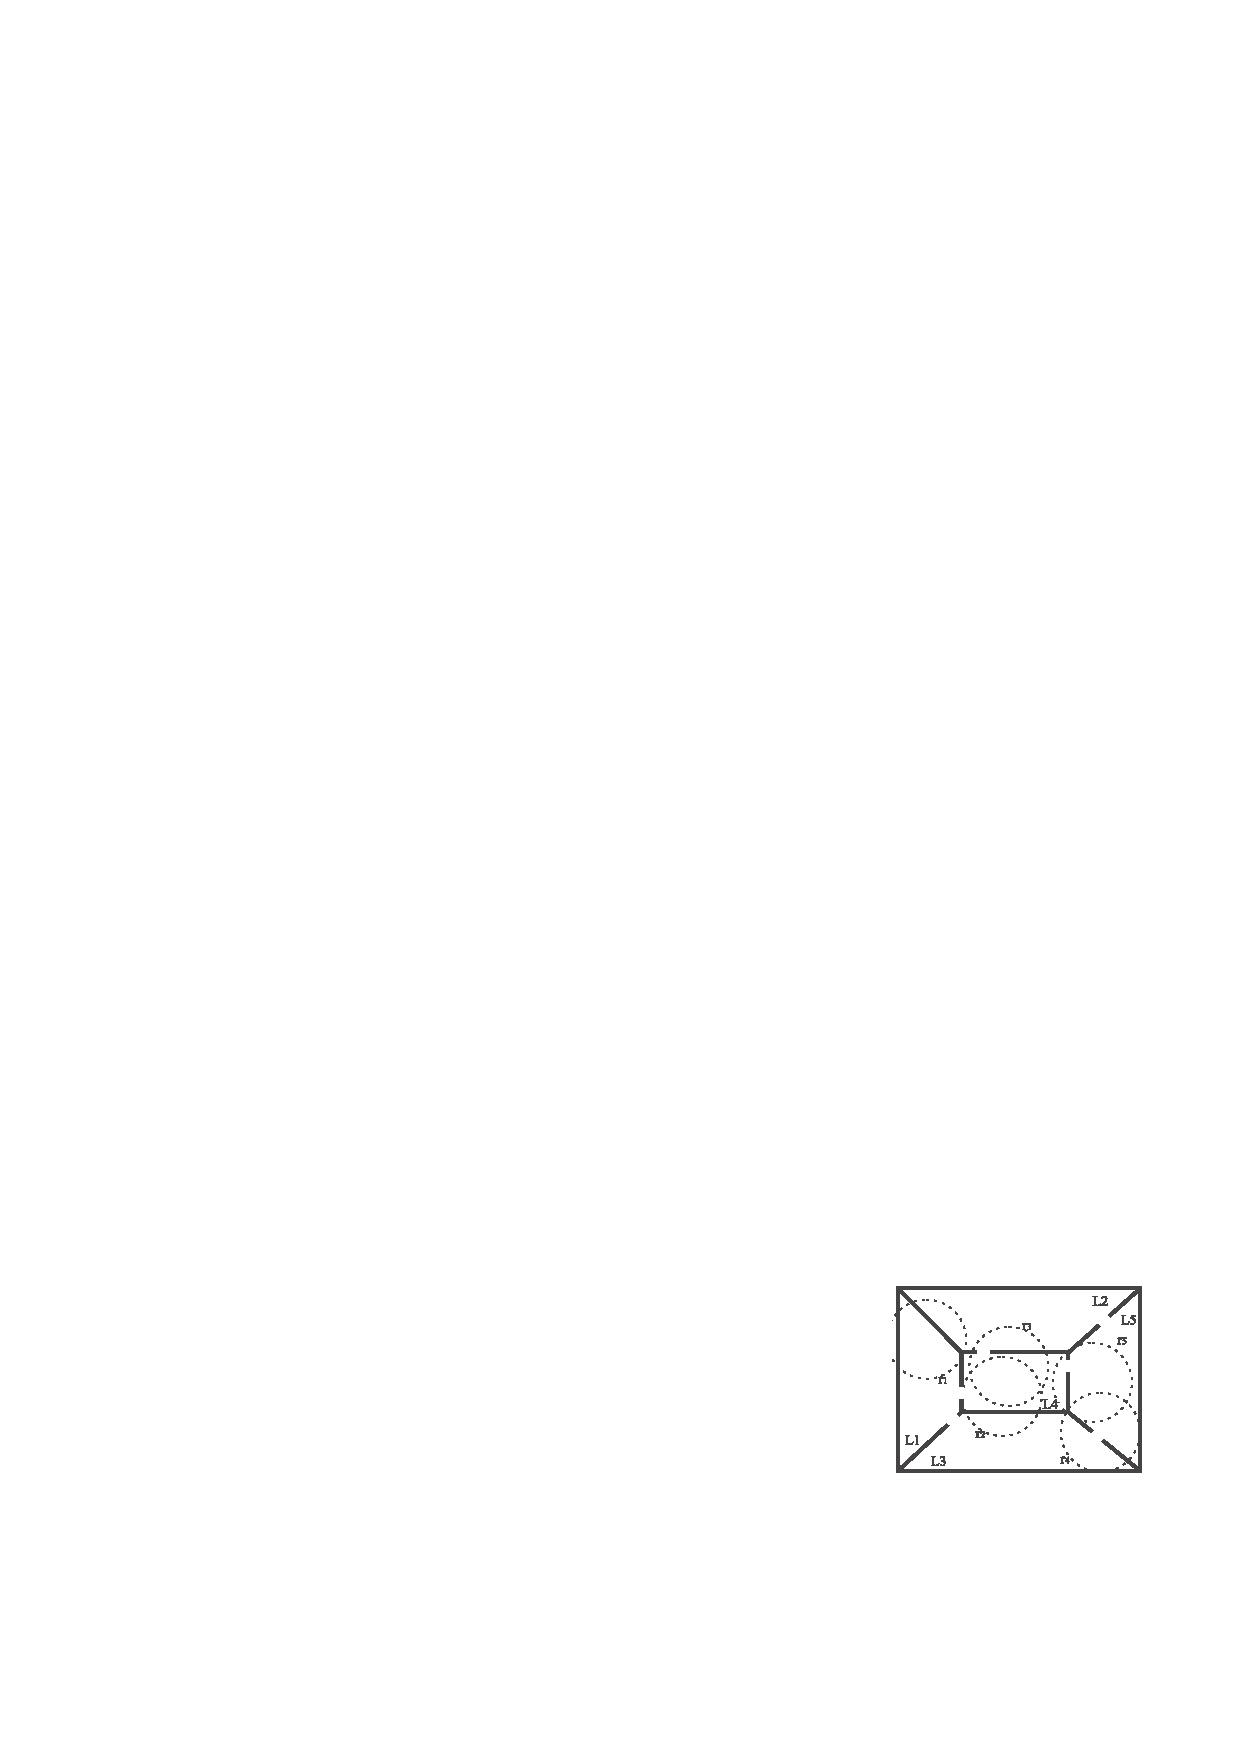
\includegraphics[width=\columnwidth]{figures/3-4/3-4-2.pdf}
  \end{figure}

  \column{0.6\textwidth}

  \begin{example}
    \ssize{
      Consider $\Gamma = \langle \Lambda,p \rangle$ and $\mathcal{IC} = \{$ $latency(L_4,2)$,$unreachable(L_2, L_3)$, $travelingTime(L_1,L_5,3) \}$, imposing that (i) if object o reaches location $L_4$, it must stay there for at least two consecutive timestamps; (ii) object $o$ cannot directly reach location $L_3$ from location $L_2$; and (iii) object $o$ cannot reach location $L_5$ from location $L_1$ in less than 3 timestamps.
    }
  \end{example}

\end{columns}

\vspace{10pt}

\fsize{\textrm{Recalling $ \Lambda = \{ \lambda_1 = \langle 0, L_1 \rangle, \lambda_2 = \langle 0, L_2 \rangle, \lambda_3 = \langle 1, L_3 \rangle, \lambda_4 = \langle 1, L_4 \rangle, \lambda_5 = \langle 2, L_3 \rangle, \lambda_6 = \langle 2, L_5 \rangle \} $, $t_1 = \{\lambda_1, \lambda_3, \lambda_5\}$ and $t_2 = \{\lambda_1, \lambda_3, \lambda_6\}$. $t_1$ is valid, as it does not violate any constraint in $\mathcal{IC}$. $t_2$ is not valid, as it does not satisfy $travelingTime(L_1, L_5, 3)$. Indeed, the difference between the timestamp of $\lambda_6$ and $\lambda_1$ is 2. It is easy to see that $t_1$ is the unique valid trajectory over $\Gamma$ and $\mathcal{IC}$.}}

\end{frame}

%------------------------------------------------

\begin{frame}
\frametitle{Maximum Traveling Time}

\begin{definition}[Maximum Traveling Time]
  Given a set $\mathcal{IC}$ of integrity constraints and a location $l \in \mathcal{L}$, we define $maxTravelingTime(l) = \max\{ \nu | travelingTime(l,l',\nu) \in \mathcal{IC} \}$, i.e., $maxTraveling(l)$ is the maximum among the minimum traveling times required for object $o$ to move from $l$ to any other $l' \in \mathcal{L}$ according to the constraints in $\mathcal{IC}$.
\end{definition}

\end{frame}

%------------------------------------------------

\begin{frame}
\frametitle{Conditioning}

\conceptbf{Conditioning}: starting from the a-priori probabilities, the probabilities of the trajectories are evaluated as conditioned to the event that the constraints are satisfied.\\~\\

\textrm{The probability of invalid trajectories becomes 0, while that of each balid trajectory becomes the ratio of its a-priori probability to the overall a-priori probability of the valid trajecories.}

\begin{block}{}
  Given a trajectory $t \in T(\Gamma)$, its probability $p^a(t)$ conditioned to the fact that the constraints in $\mathcal{IC}$ are satisfied is given by $p^a(t|\mathcal{IC})$, where:

  \begin{itemize}
    \item $p^a(t|\mathcal{IC}) = 0$ if $t$ is not valid w.r.t $\mathcal{IC}$;
    \item $p^a(t|\mathcal{IC}) = \frac{p^a(t)}{\sum_{t' \in T^{\models \mathcal{IC}}(\Gamma)} p^a(t')}$, otherwise.
  \end{itemize}

\end{block}

\end{frame}

%------------------------------------------------

\begin{frame}
\frametitle{Conditioned Trajectory Graphs}

The \conceptbf{conditioned trajectory graph} (ct-graph) over an l-sequence $\Gamma = \langle \Lambda,p \rangle$ will be exploited to concisely represent trajectories over $\Gamma$ in the presence of integrity constraints.\\~\\

The nodes of a ct-graph are said to be \emph{location nodes}, each location node $n$ corresponds to a pair $\langle \tau,l \rangle \in \Lambda$ and is connected through directed edges to location nodes (chosen among the set of \emph{successors} of $n$) corresponding to sbusequent timestamps.

\end{frame}

%------------------------------------------------

\begin{frame}
\frametitle{Location Nodes}

\begin{definition}[Location Nodes]
  Given an l-sequence $\Gamma = \langle \Lambda,p \rangle$ for an object $o$ and a set $\mathcal{IC}$ of intergrity constraints, a location node $n$ is a tuple of the form $\langle \tau, l, \delta, TL \rangle$, where $\langle \tau, l \rangle \in \Lambda$, $\delta \in \mathcal{T} \cup \{ \perp \}$ (where $\perp$ means ``non-specified''), and $TL$ is a (possible empty) set of pairs $\langle \tau_1, l_1 \rangle \in \Lambda$ (with $l_1 \neq l$) containing no two pairs conciding in either the timestamp or the location. It represents the following facts:
  \begin{enumerate}
    \item A. $o$ was in location $l$ at time $\tau$;
    \item B. the stay of $o$ at $l$ started $\delta$ time points before $\tau$;
    \item C. for each $\langle \tau_1, l_1 \rangle \in TL$, the most recent detection of $o$ at location $l_1$ (before $\tau$) is at time point $\tau_1$.
  \end{enumerate}
\end{definition}

\end{frame}

%------------------------------------------------

\begin{frame}
\frametitle{Location Nodes}

Given a location node $n = \langle \tau, l, \delta, TL \rangle$ and a trajectory $t$ over $\Gamma$, we say that $t$ \conceptbf{is compatible with} $n$ if, according to $t$, the facts A,B,C holds.\\~\\

E.g., both the trajectories $t_1 = \{ \langle 0,L_1 \rangle, \langle 1,L_3 \rangle, \langle 2,L_3 \rangle \}$ and $t_2 = \{ \langle 0,L_1 \rangle, \langle 1,L_3 \rangle, \langle 2,L_5 \rangle \}$ are compatible with location node $\langle 1, L_3, 0, \{ \langle 0, L_1 \rangle \} \rangle$.

\end{frame}

%------------------------------------------------

\begin{frame}
\frametitle{Location Nodes}

The information stored in a location node $n$ can be used to state that some trajectories are invalid. Specifically, any $t \in T(\Gamma)$ compatible with $n$ is invalid if either i) or ii) hold:

\begin{block}{}
  \fsize{
  i) All the following conditions are satisfied:
  \begin{itemize}
    \item $n.TL$ contains a pair $\langle \tau', l' \rangle$;
    \item there is $travelingTime(l', l'', \nu') \in \mathcal{IC}$ with $(n.\tau+1) - \tau' < \nu'$;
    \item the $(\tau+1)$-th step of $t$ is at location $l''$.
  \end{itemize}
  In fact, $t$ would represent that the object went from $l'$ to $l''$ in less than $\nu'$ time points, thus violating the $TT$ constraints.\\~\\

  ii) There is $latency(l, \delta') \in \mathcal{IC}$ with $n.\delta < \delta'$, and the $(\tau+1)$-step of $t$ is at a location different from $l$. In fact, $t$ would represent that the object went away from $l$ after staying less than $\delta'$ time points, thus violating the latency constraint.
  }
\end{block}

\end{frame}

%------------------------------------------------

\begin{frame}
\frametitle{Location Nodes}

\fsize{
E.g., consider location node $n = \{ \langle 1, L_3, 0, \{ \langle 0, L_1 \rangle \} \rangle \}$ and the $TT$ constraint $travelingTime(L_1, L_5, 3)$. It is easy to see that the information stored in $n$ can be used to state that any trajectory compatible with $n$ and whose second step is at $L_5$ is invalid. (would not reach location $L_5$ from $L_1$ in less than 3 timestamps).\\~\\

Point i) means that an entry $\langle \tau',l' \rangle$ in $n.TL$ can be used only to check $TT$ constraints involving location $l'$. Point ii) means that the value of $n.\delta$ is useful only to check latency constraints defined over $l$.\\~\\

$\mathcal{N}$ is denoted as the set of the location nodes that can be defined over $\Gamma$ and $\mathcal{IC}$. $SN$ AND $TN$ is the subsets of $\mathcal{N}$ as the \emph{source} and \emph{target} nodes (location nodes whose timestamps are the first and the last time points of $\mathcal{T}$), respectively.
}

\end{frame}

%------------------------------------------------

\begin{frame}
\frametitle{Location Nodes}

\begin{columns}

  \column{0.4\textwidth}
  \begin{figure}[tb]
    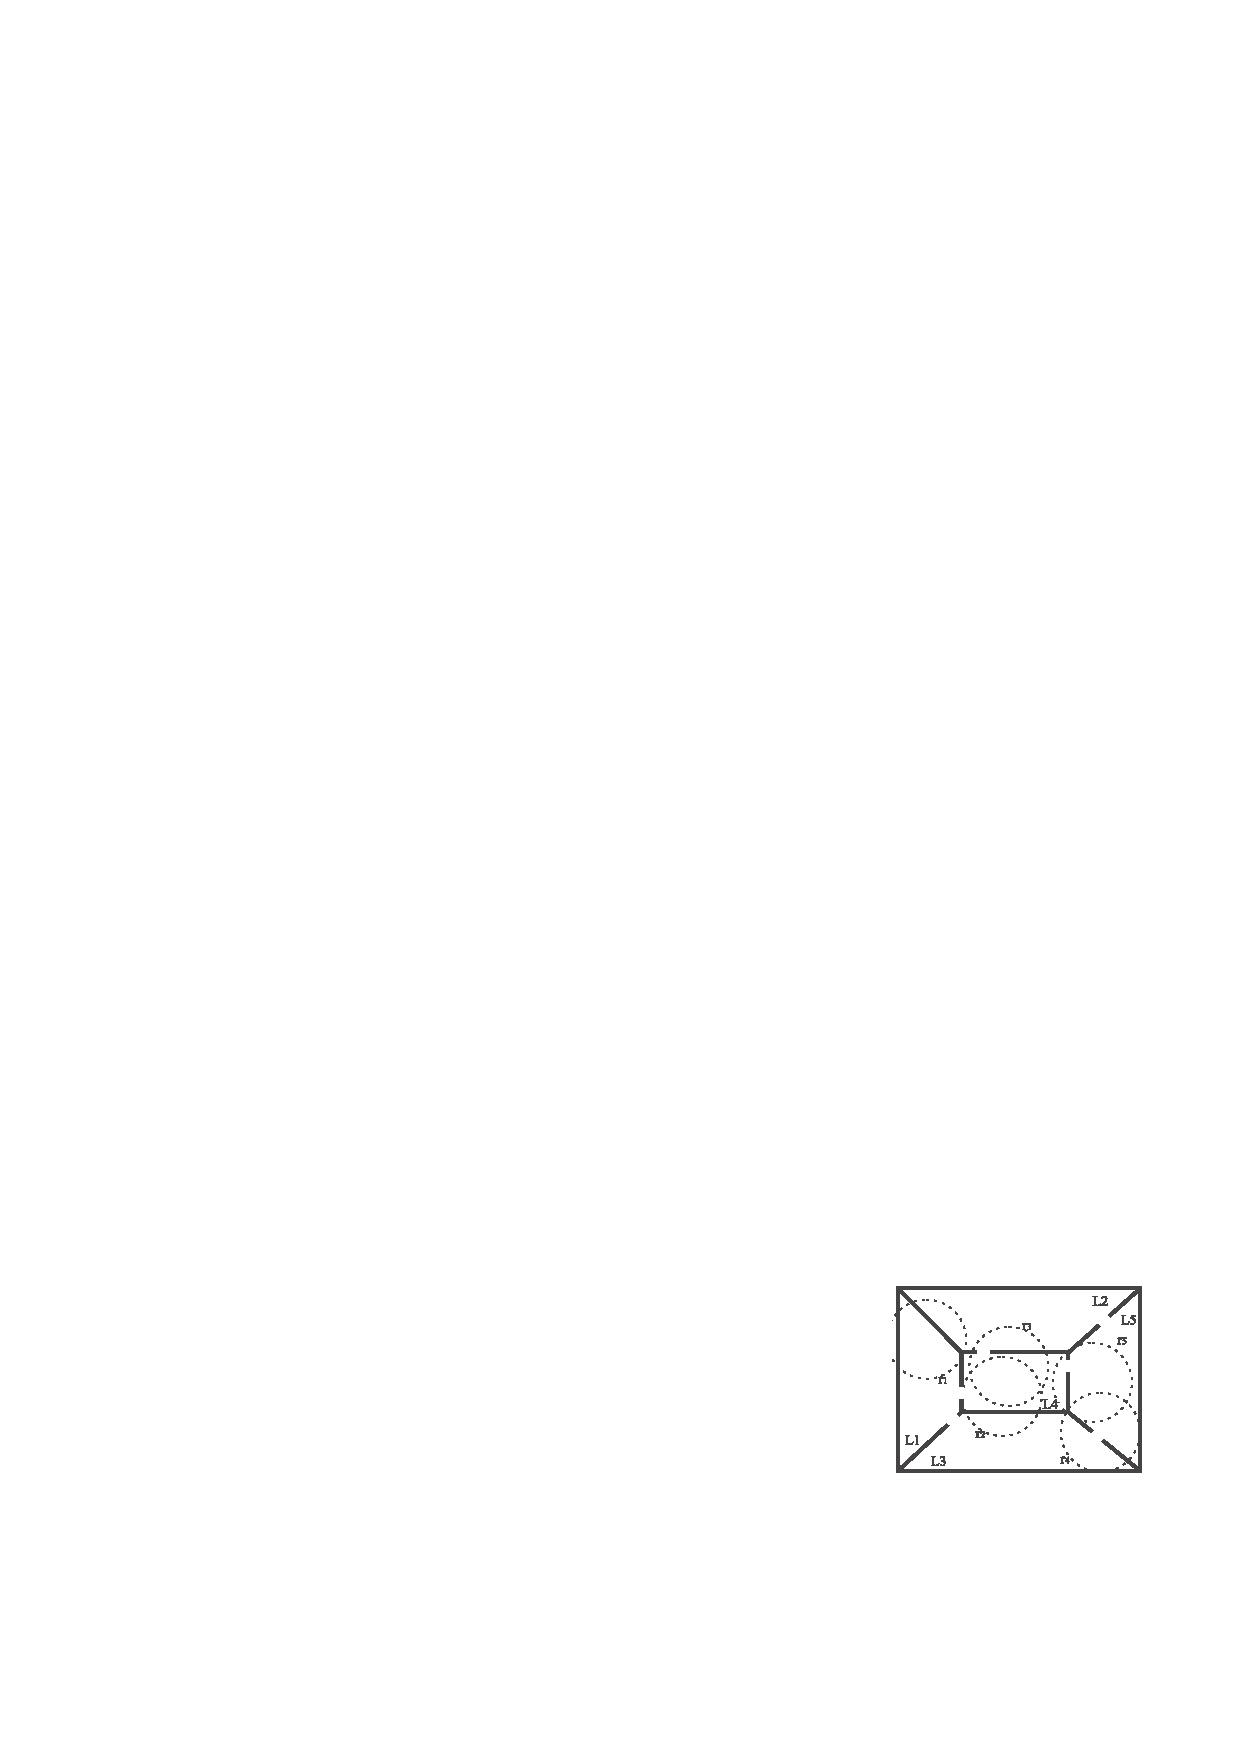
\includegraphics[width=\columnwidth]{figures/3-4/3-4-2.pdf}
  \end{figure}

  \column{0.6\textwidth}

  \begin{example}
    \ssize{
      Consider the set $\mathcal{N}$ over $\Gamma$ and $\mathcal{IC}$ consists of the following location nodes:\\
      $n_0 = \langle 0, L_1, \perp, \varnothing \rangle$, $n_1 = \langle 0, L_2, \perp, \varnothing \rangle$ \\
      $n_2 = \langle 1, L_3, \perp, \varnothing \rangle$, $n_3 = \langle 1, L_3, \perp, \{ \langle 0, L_1 \rangle \} \rangle$ \\
      $n_4 = \langle 1, L_4, 0, \varnothing \rangle$, $n_5 = \langle 1, L_4, 0, \{ \langle 0, L_1 \rangle \} \rangle$ \\
      $n_6 = \langle 2, L_3, \perp, \varnothing \rangle$, $n_7 = \langle 2, L_3, \perp, \{ \langle 0, L_1 \rangle \} \rangle$ \\
      $n_8 = \langle 2, L_5, \perp, \varnothing \rangle$, $n_9 = \langle 2, L_5, \perp, \{ \langle 0, L_1 \rangle \} \rangle$
    }
  \end{example}

\end{columns}

\end{frame}

%------------------------------------------------

\begin{frame}
\frametitle{Location Nodes}

\LARGE
$$n_2 = \langle 1, L_3, \perp, \varnothing \rangle$$

\vspace{10pt}

\fsize{
Location node $n_2$ means that:

\begin{fitemize}

  \item since $n_2.\tau = 1$ and $n_2.l = L_3$, $o$ was in $L_3$ at timestamp 1;

  \item since $n_2.\delta = \perp$, either there is no $LT$ constraint over $L_3$, or its stay at $L_3$ started more than $\delta^*$ time points before 1, where $latency(L_3, \delta^*)$ is the $LT$ constraint over $L_3$;

  \item since $n_2.TL = \varnothing$, for every location $l$ visited by the object in the past, either there is no $TT$ constraints having $l$ as the firt argument, or the object left $l$ more than $\nu^*$ time points ago, where all the $TT$ constraints $travelingTime(l,l',\nu) \in \mathcal{IC}$ having $l$ as first argument are such that $\nu < \nu^*$.

\end{fitemize}

}

\end{frame}

%------------------------------------------------

\begin{frame}
\frametitle{Location Nodes}

\LARGE
$$n_5 = \langle 1, L_4, 0, \{ \langle 0, L_1 \rangle \} \rangle$$

\vspace{10pt}

\fsize{
Location node $n_5$ means that:

\begin{fitemize}

  \item $o$ was in $L_4$ at timestamp 1;

  \item its stay at $L_4$ started in the current timestamp;

  \item in the past, it stayed at $L_1$, from which it moved away at time point 0.

\end{fitemize}

}

\end{frame}

%------------------------------------------------

\begin{frame}
\frametitle{Successors of a Location Node}

\ssize{
\begin{definition}[Successor]
  Given a pair of location nodes $n_1 = \langle \tau_1, l_1, \delta_1, TL_1 \rangle$ and $n_2 = \langle \tau_2, l_2, \delta_2, TL_2 \rangle$, $n_2$ is successor of $n_1$ iff the following conditions hold:
  \begin{itemize}
    \item $\tau_2 = \tau_1 + 1$;
    \item $unreachable(l_1, l_2) \notin \mathcal{IC}$;
    \item if $l_1 = l_2$, then $\delta_2 = \delta_1 + 1$  (override ``+'': $\perp + 1 = \perp$; $x+1 = \perp$);
    \item if $l_1 \neq l_2$, and $latency(l_1, \delta) \in \mathcal{IC}$, then $\delta_1 \leq \delta$ (if $\delta_1 \neq \perp$) and either $\delta_2 = 0$ (if there is a latency constraint on $l_2$ in $\mathcal{IC}$) or $\delta_2 = \perp$ (otherwise);
    \item there is no pair $(\tau', l') \in TL_1$ such that there is a constraint $travelingTime(l',l_2,\nu)$ in $\mathcal{IC}$ with $\tau_2 - \tau' < \nu$;
    \item $TL_2 = TL_1 \cup \{ \langle \tau_1,l_1 \rangle | travelingTime(l_1,l,\delta) \in \mathcal{IC} \} \setminus$ $(\{ \langle \tau,l \rangle \in TL_1 | \tau_2 - \tau \leq maxTravelingTime(l) \} \cup \{ \langle \tau,l \rangle \in TL_1 | l = l_2 \})$
  \end{itemize}
\end{definition}
}
\end{frame}

%------------------------------------------------

\begin{frame}
\frametitle{Successors of a Location Node}

$n_2$ is a successor of $n_1$ iff:

\begin{fitemize}
  \item $n_1$ and $n_2$ refer to consecutive time points;
  \item $l_2$ can be directly reached starting from $l_1$;
  \item if at time $\tau_2$ the object is still in $l_2 = l_1$, then this is consistently reflected by an increment of $\delta_2$;
  \item no stay constraint in $\mathcal{IC}$ involving $l_1$ is violated if the object moves from $l_1$ to another location $l_2$ at time $\tau_2$;
  \item no traveling time constraint in $\mathcal{IC}$ imposing that the time needed to move from a location belonging to $TL_1$ to $l_2$ is violated if the object moves from $l_1$ to another location $l_2$ at time $\tau_2$;
  \item $TL_2$ can be obtained by first angumenting $TL_1$ with the pair $\langle \tau_1, l_1 \rangle$ (this happens if there is a traveling time constraint involving $l_1$ as the first argument), and discarding those pairs of $TL_1$ which have become useless for checking $TT$ constraint and those referring to a previous stay at $l_2$.
\end{fitemize}

\end{frame}

%------------------------------------------------

\begin{frame}
\frametitle{Successors of a Location Node}

\begin{center}
  $n_0 = \langle 0, L_1, \perp, \varnothing \rangle$, $n_1 = \langle 0, L_2, \perp, \varnothing \rangle$ \\
  $n_2 = \langle 1, L_3, \perp, \varnothing \rangle$, $n_3 = \langle 1, L_3, \perp, \{ \langle 0, L_1 \rangle \} \rangle$ \\
  $n_4 = \langle 1, L_4, 0, \varnothing \rangle$, $n_5 = \langle 1, L_4, 0, \{ \langle 0, L_1 \rangle \} \rangle$ \\
  $n_6 = \langle 2, L_3, \perp, \varnothing \rangle$, $n_7 = \langle 2, L_3, \perp, \{ \langle 0, L_1 \rangle \} \rangle$ \\
  $n_8 = \langle 2, L_5, \perp, \varnothing \rangle$, $n_9 = \langle 2, L_5, \perp, \{ \langle 0, L_1 \rangle \} \rangle$
\end{center}

\begin{example}
  $n_3$ and $n_5$ are successors of $n_0$, $n_4$ is a successor of $n_1$, $n_7$ is a successor of $n_3$.\\
  $n_2$ is not a successor of $n_1$ since $unreachable(L_2,L_3) \in \mathcal{IC}$; $n_9$ is not a successor of $n_3$ since $travelingTime(L_1, L_5, 3) \in \mathcal{IC}$; $n_9$ is not a successor of $n_2$ for both $TT$ constraints and the previous stay conditions.
\end{example}


\end{frame}

%------------------------------------------------

\begin{frame}
\frametitle{Successors of a Location Node}

\textrm{The following proposition states a property that will be fundamental for understanding how cleansing algorithm exploits the notion of successor.}\\~\\

\begin{block}{Proposition}
  If a non-target location node $n$ admits no successor then every trajectory $t$ compatible with $n$ is not valid.
\end{block}

\end{frame}

%------------------------------------------------

\begin{frame}
\frametitle{CT-Graph}

\begin{definition}[CT-Graph]
  Let $\mathcal{N}$ be the set of location nodes over the l-sequence $\Gamma$, and $\mathcal{IC}$ a set of integrity constraints. A conditioned trajectory graph (ct-graph) is a tuple $G = \langle N, E, p_N, \vec{p}_E \rangle$:
  \begin{fitemize}
    \item $N \subseteq \mathcal{N}$;
    \item $\langle N,E \rangle$ is a graph (where $N$ and $E$ are the sets of nodes and edges, respectively) satisfying the following properties
      \begin{sitemize}
        \item a pair $\langle n_1, n_2 \rangle$ belongs to $E$ iff $n_1, n_2 \in N$ and $n_2$ is a successor of $n_1$;
        \item for every $n \in N$, there is at least one path from a source node to a target node in $N$ which contains $n$.
      \end{sitemize}
    \item $p_N: SN \rightarrow (0, 1]$ is a PDF over the set of source nodes;
    \item $\vec{p}_E$ is a set containing, for each non-target node $n$ of $G$, a PDF $p^n_E$ over its outgoing edges, i.e., $\vec{p}_E = \{ p^n_E | n \in N \setminus TN \}$ where $p^n_E: E_n \rightarrow (0,1]$ and $E_n = \{ \langle n, n' \rangle | \langle n, n' \rangle \in E \}$
  \end{fitemize}
\end{definition}

\end{frame}

%------------------------------------------------

\begin{frame}
\frametitle{CT-Graph}

A (valid) path $\pi$ over a ct-graph $G = \langle N,E,p_N,\vec{p}_E \rangle$ is a path from a source to a target node over the graph $\langle N,E \rangle$.\\~\\

A path $\pi = n_0, ..., n_{\tau_f}$ over $G$ corresponds to the valid trajectory $t = n_0[\lambda],...,n_{\tau_f}[\lambda]$, where $n_i[\lambda]$ denotes the $\langle timestamp, location \rangle$ pair which $n_i$ refers to.\\~\\

The functions $p_N$ and $\vec{p}_E$ is equal to the conditioned probability $p^a(t | \mathcal{IC})$ of the corresponding trajectory $t$, where
\begin{equation}
  p(\pi) = p_N(n_0) \times \prod_{i=0}^{\tau_f-1}p_E^{n_i}(\langle n_i, n_{i+1} \rangle)
\end{equation}

\end{frame}

%------------------------------------------------

\begin{frame}
\frametitle{Location Nodes}

\begin{columns}

  \column{0.4\textwidth}
  \begin{figure}[tb]
    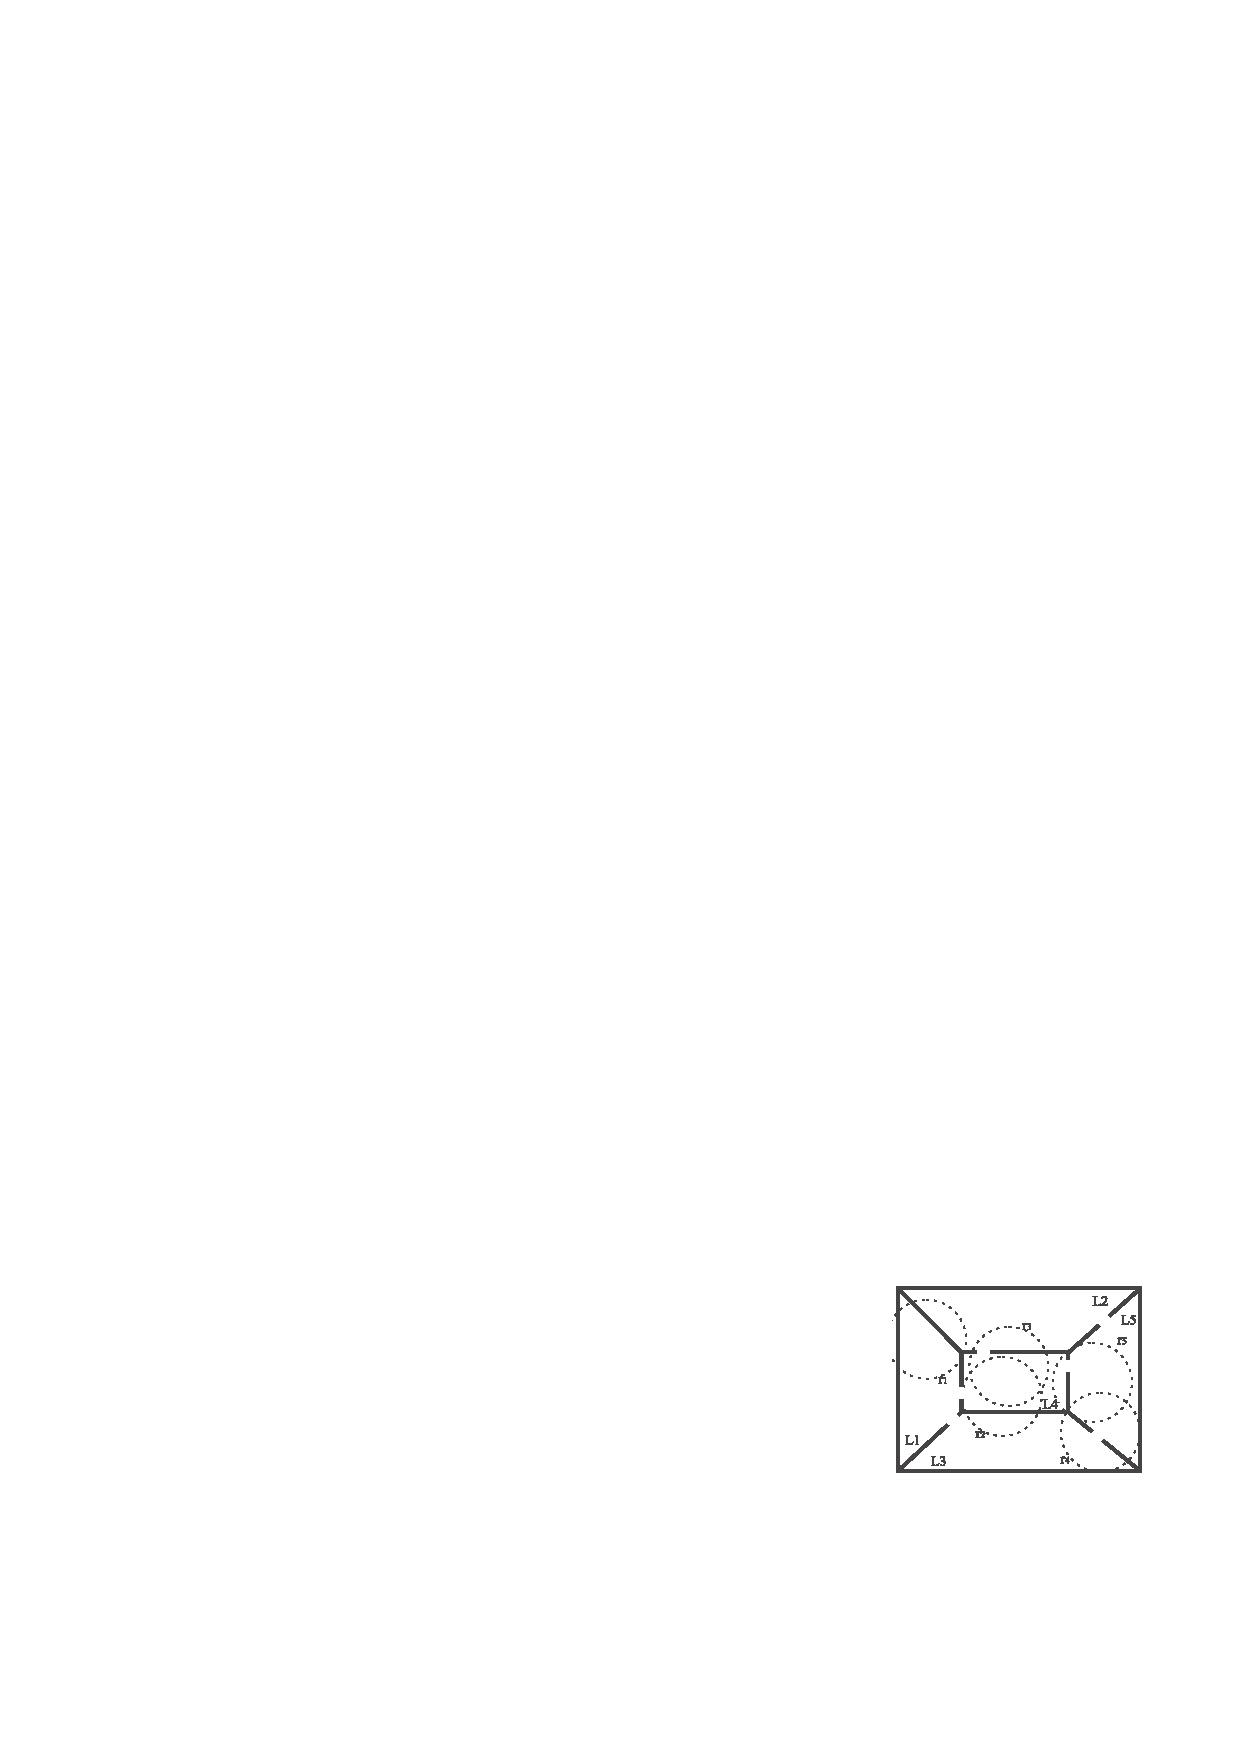
\includegraphics[width=\columnwidth]{figures/3-4/3-4-2.pdf}
  \end{figure}

  \column{0.6\textwidth}

  \begin{example}
    \ssize{
      It is easy to check $G = \langle N,E,p_N,\vec{p}_E \rangle$, where $N = \{ n_0, n_3, n_7 \}$, $E= \{ \langle n_0,n_3 \rangle, \langle n_3,n_7 \rangle \}$, $p_N(n_0) = 1$, and $p_E^{n_3}(\langle n_3, n_7 \rangle) = 1$. $G$ is the ct-graph over the l-sequence and the constraints. In fact, the unique path $\pi = n_0, n_3, n_7$ over $G$ corresponds to the unique valid trajectory $\{ \lambda_1, \lambda_3, \lambda_5 \}$, and its probability is $p(\pi) = 1$.
    }
  \end{example}

\end{columns}

\end{frame}

%------------------------------------------------

\begin{frame}
\frametitle{The Cleansing Algorithm: Overview}

\begin{columns}

  \column{0.4\textwidth}
  \begin{figure}[tb]
    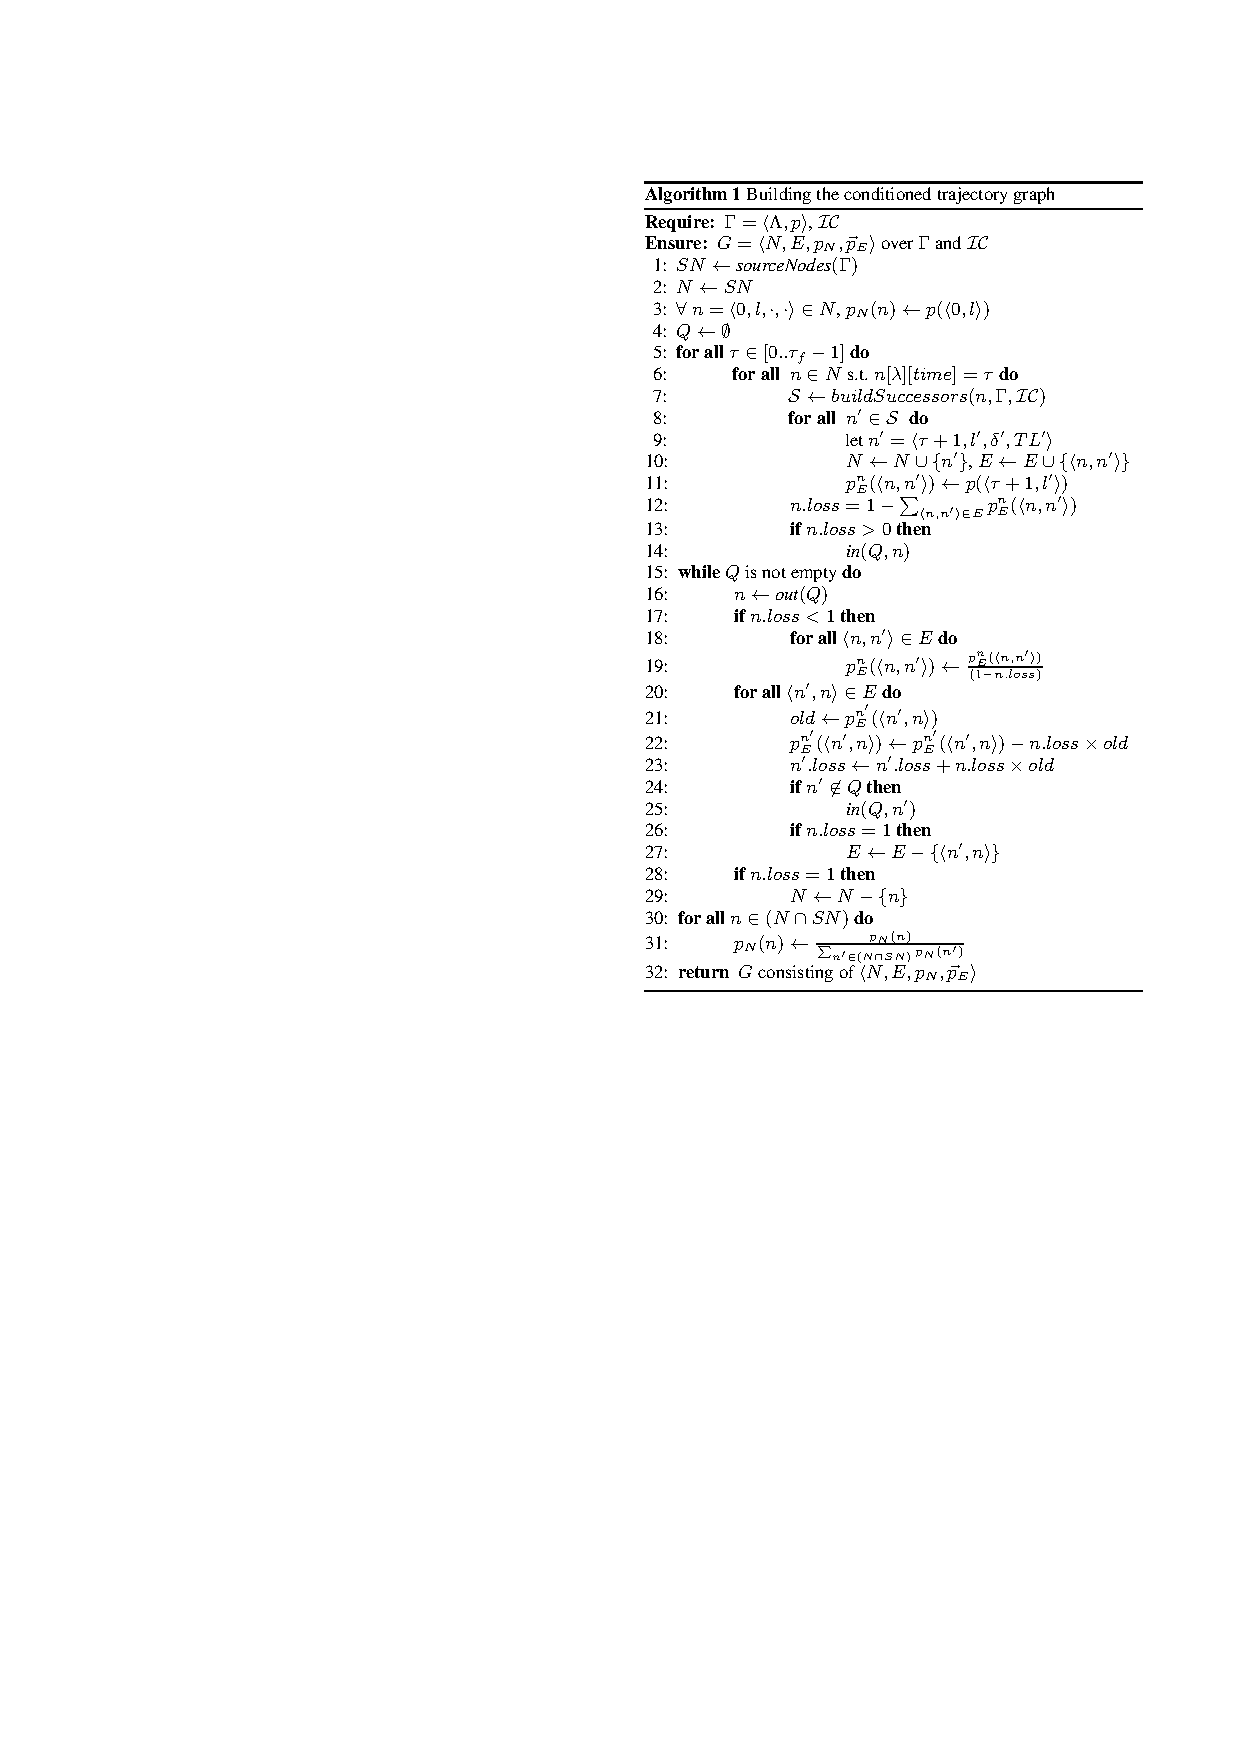
\includegraphics[width=\columnwidth]{figures/3-4/3-4-3.pdf}
  \end{figure}

  \column{0.6\textwidth}
  \begin{sitemize}
    \item consists of \emph{forward} and \emph{backward} phase;
    \item the forward phase consists of one iteration for each timestamp $\tau \in \mathcal{T}$, at the first iteration, the set $N$ of the location nodes belonging to the ct-graph $G$ being constructed is initialized with the set to those implied by the a-priori probabilities.
    \item at $\tau$-th iteration, $N$ is progressively augmented with location nodes referring to the timestamp $\tau+1$, the edges between location nodes reffering to timestamp $\tau$ and their successors are added to $E$, and their probabilities are set to those implied by the a-priori probability function.
    \item the backward phase deals with removing the nodes in the invalid paths, the probabilities of edges and those of source nodes are conditioned, i.e., they are revised to take into account the probabilities of the trajectories that are invalid.
  \end{sitemize}

\end{columns}

\end{frame}

%------------------------------------------------

\begin{frame}
\frametitle{The Cleansing Algorithm: Initialization}

\begin{columns}

  \column{0.42\textwidth}
  \begin{figure}[tb]
    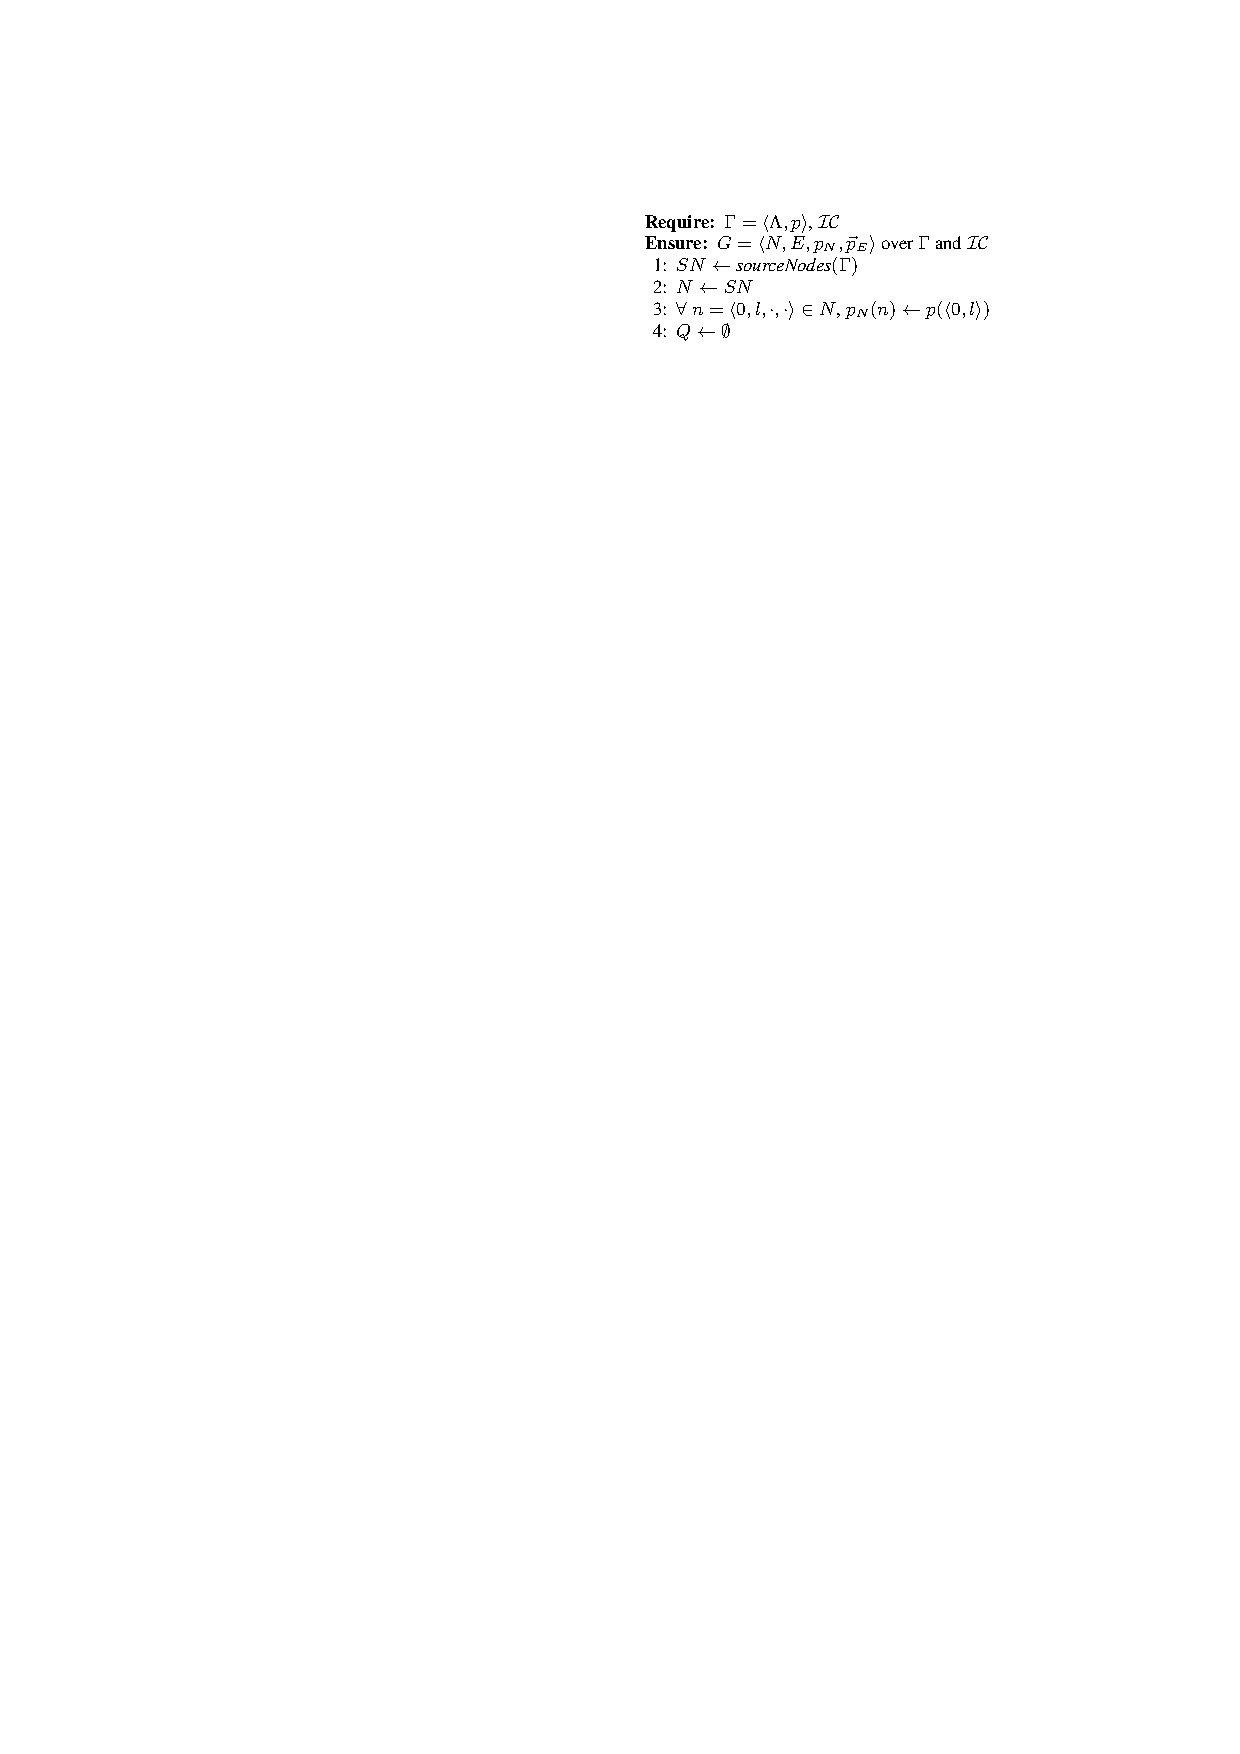
\includegraphics[width=\columnwidth]{figures/3-4/3-4-4.pdf}
  \end{figure}

  \column{0.58\textwidth}
  \begin{enumerate}
    \ssize{
    \item lines 1--2: the set $N$ if the nodes of graph is initialized with the set of the source nodes yielded by funtion \emph{sourceNodes} that builds them from the l-sequence $\Gamma$.
    \item lines 3--4: the probability $p_N(n)$ of each source node $n$ is set to the probability of the pair $\langle 0,l\rangle$ of $\Gamma$, and the queue $Q$ is set to be empty.
    }
  \end{enumerate}

\end{columns}

\begin{example}
  according to the previous example, function \emph{sourceNodes} builds the source location nodes $n_0$ and $n_1$, and puts them into $N$. Next, $p_N(n_0)$ and $p_N(n_1)$ are assigned probabilities $p(\lambda_1) = \frac{6}{10}$ and $p(\lambda_2) = \frac{4}{10}$, respectively.
\end{example}

\end{frame}

%------------------------------------------------

\begin{frame}
\frametitle{The Cleansing Algorithm: Forward Phase}

\begin{columns}

  \column{0.5\textwidth}
  \begin{figure}[tb]
    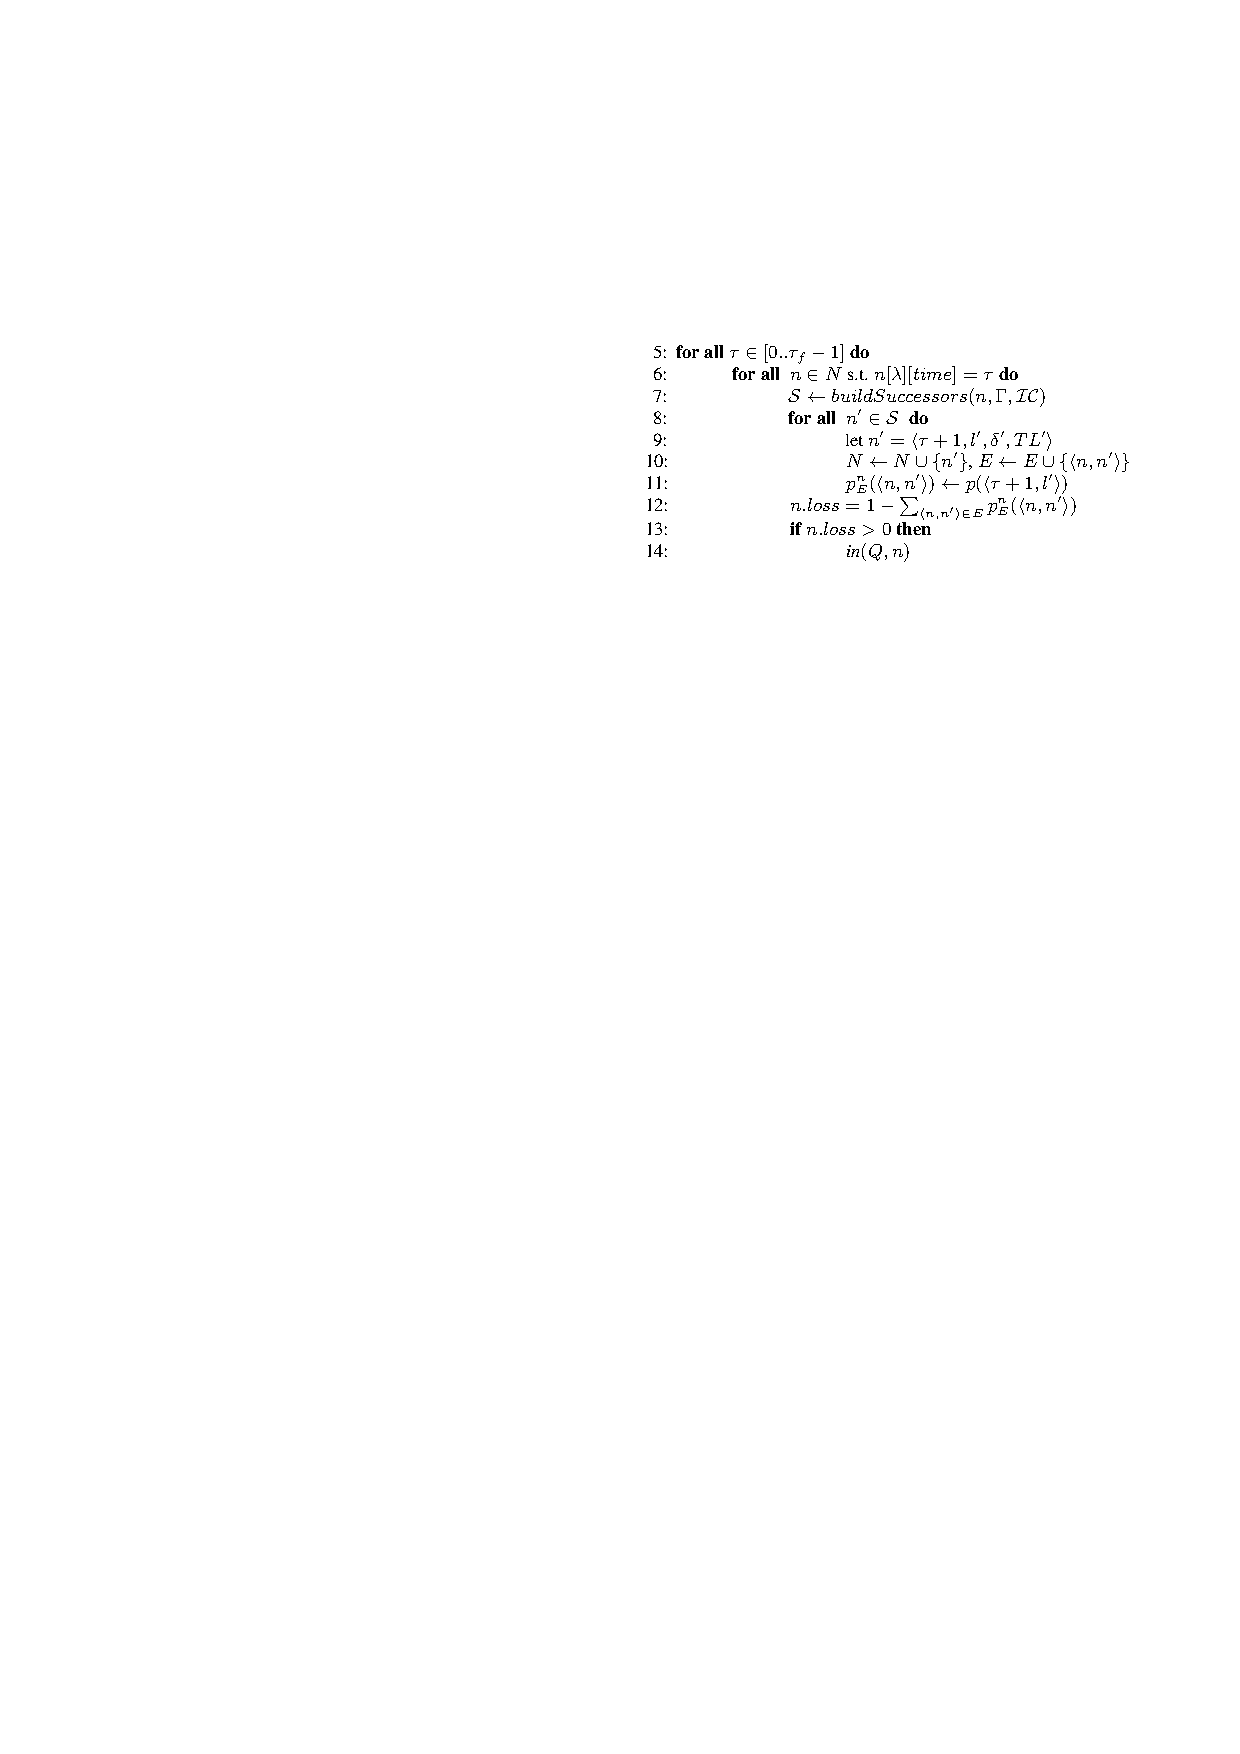
\includegraphics[width=\columnwidth]{figures/3-4/3-4-5.pdf}
  \end{figure}

  \column{0.5\textwidth}
  \begin{enumerate}
    \ssize{
    \item line 7: for each location node $n$ referring to $\tau$, \emph{buildSuccessors} returns the its successor $n'$;
    \item line 10: each node $n'$ is added to $N$ and consequently the edges of the form $\langle n, n' \rangle$ are added to the set $E$ of $G$;
    \item line 12: once all successors have been added to $G$, $n.loss$ is set to the one's complement of the sum of the probabilities of the outgoing edge of $n$.
    }
  \end{enumerate}

\end{columns}

\end{frame}

%------------------------------------------------

\begin{frame}
\frametitle{The Cleansing Algorithm: Forward Phase}

\begin{figure}[tb]
  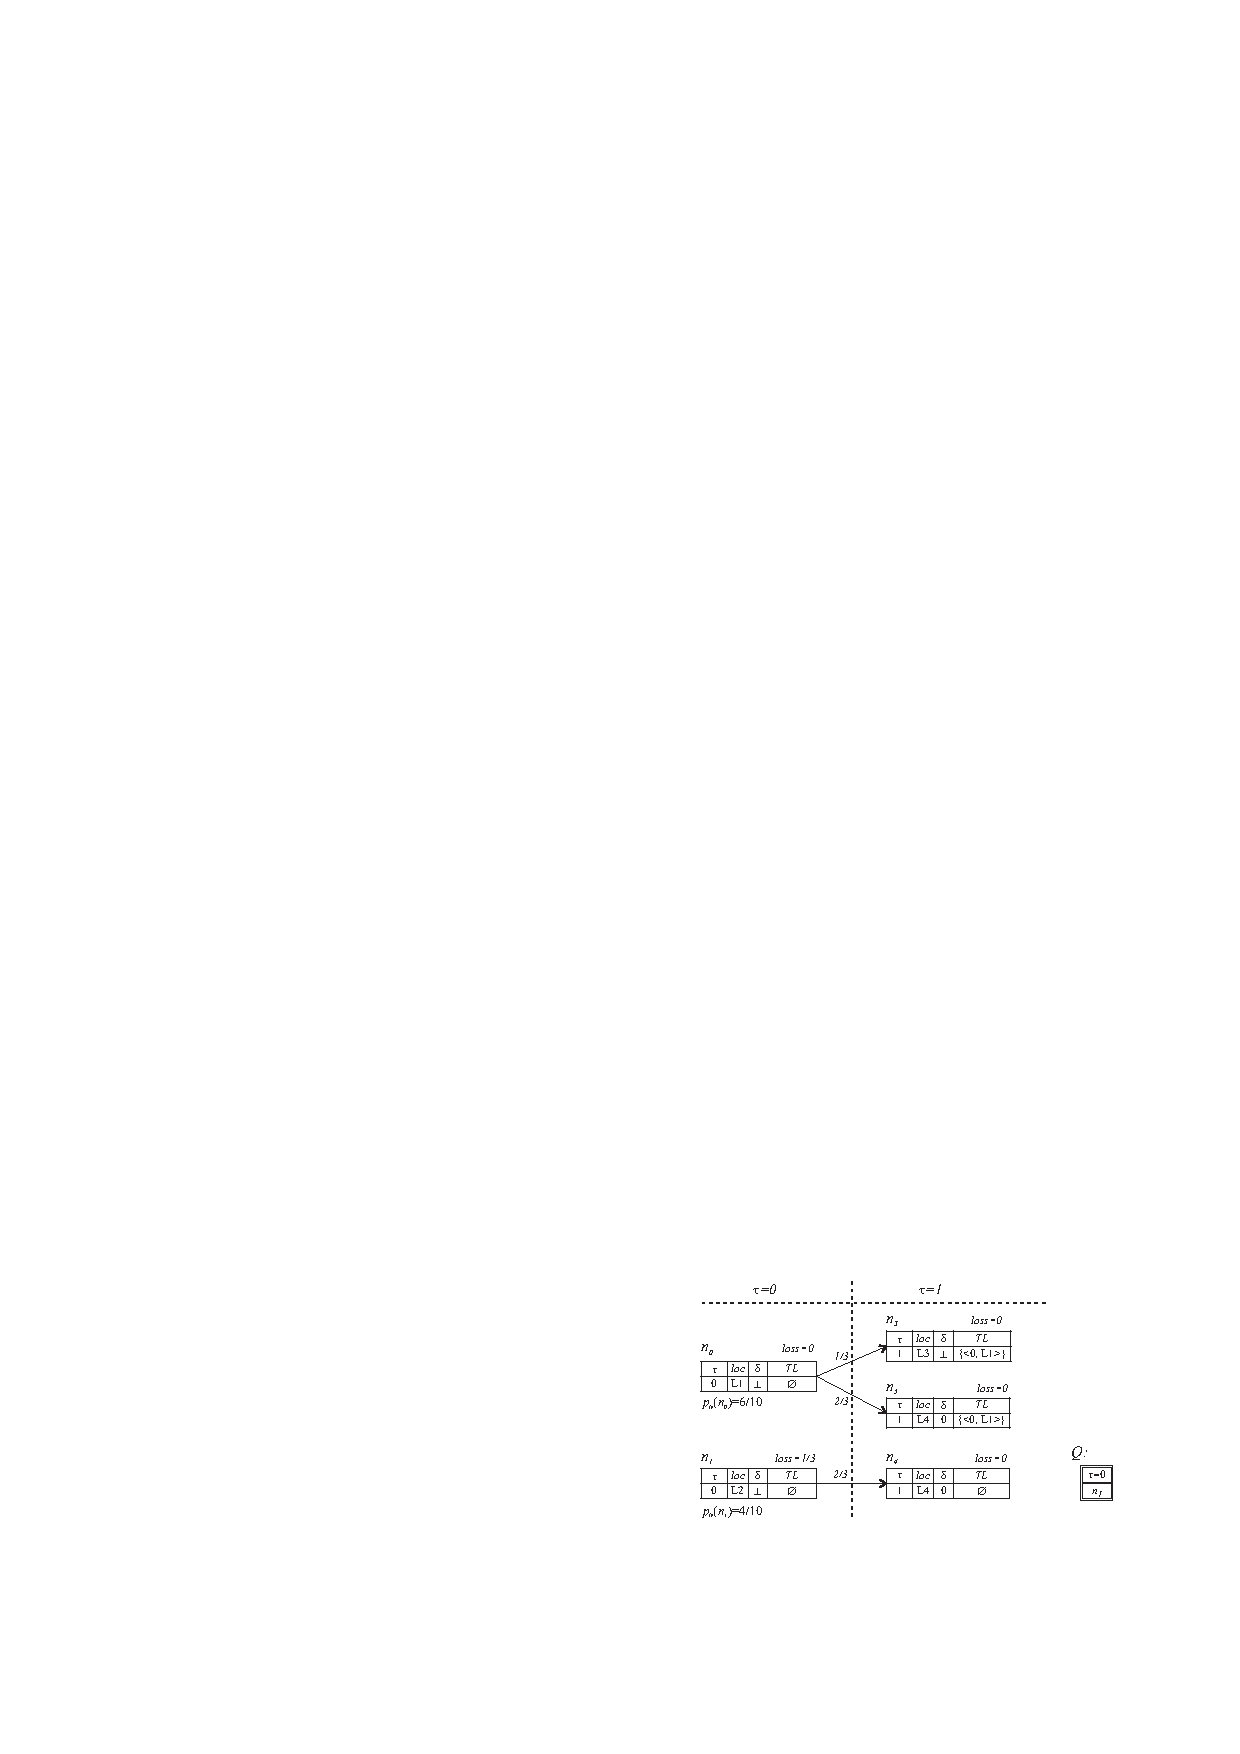
\includegraphics[width=0.5\columnwidth]{figures/3-4/3-4-6.pdf}
\end{figure}

\vspace{-15pt}

\begin{example}
  \ssize{
  At iteration $\tau = 0$, both $n_0$ and $n_1$ are processed. In the case $n=n_0$, the inner loop processes the location nodes $n_3$ and $n_5$, both nodes $n_3$ and $n_5$ are sucessors of $n_0$, and both $\langle n_0,n_3 \rangle$ and $\langle n_0,n_5 \rangle$ are added to $E$, with probabilities $p(\langle n_0,n_3 \rangle) = p(\langle 1,L_3 \rangle) = 1/3$ and $p(\langle n_0,n_5 \rangle) = p(\langle 1,L_4 \rangle) = 2/3$. At the end of the loop, $n_0.loss$ is 0 and thus $n_0$ is not added to $Q$. \\
  Another example, $n_2$ is not a successor of $n_0$ or $n_1$, in the case $n=n_1$, the loop only processes the location node $n_4$, the probability $p(\langle n_1,n_4 \rangle) = p(\langle 1, L_4\rangle) = 1/3$, and $n_1.loss = 1 - 1/3 = 2/3$, thus $n_1$ is added to $Q$.
  }
\end{example}

\end{frame}

%------------------------------------------------

\begin{frame}
\frametitle{The Cleansing Algorithm: Forward Phase}

\begin{figure}[tb]
  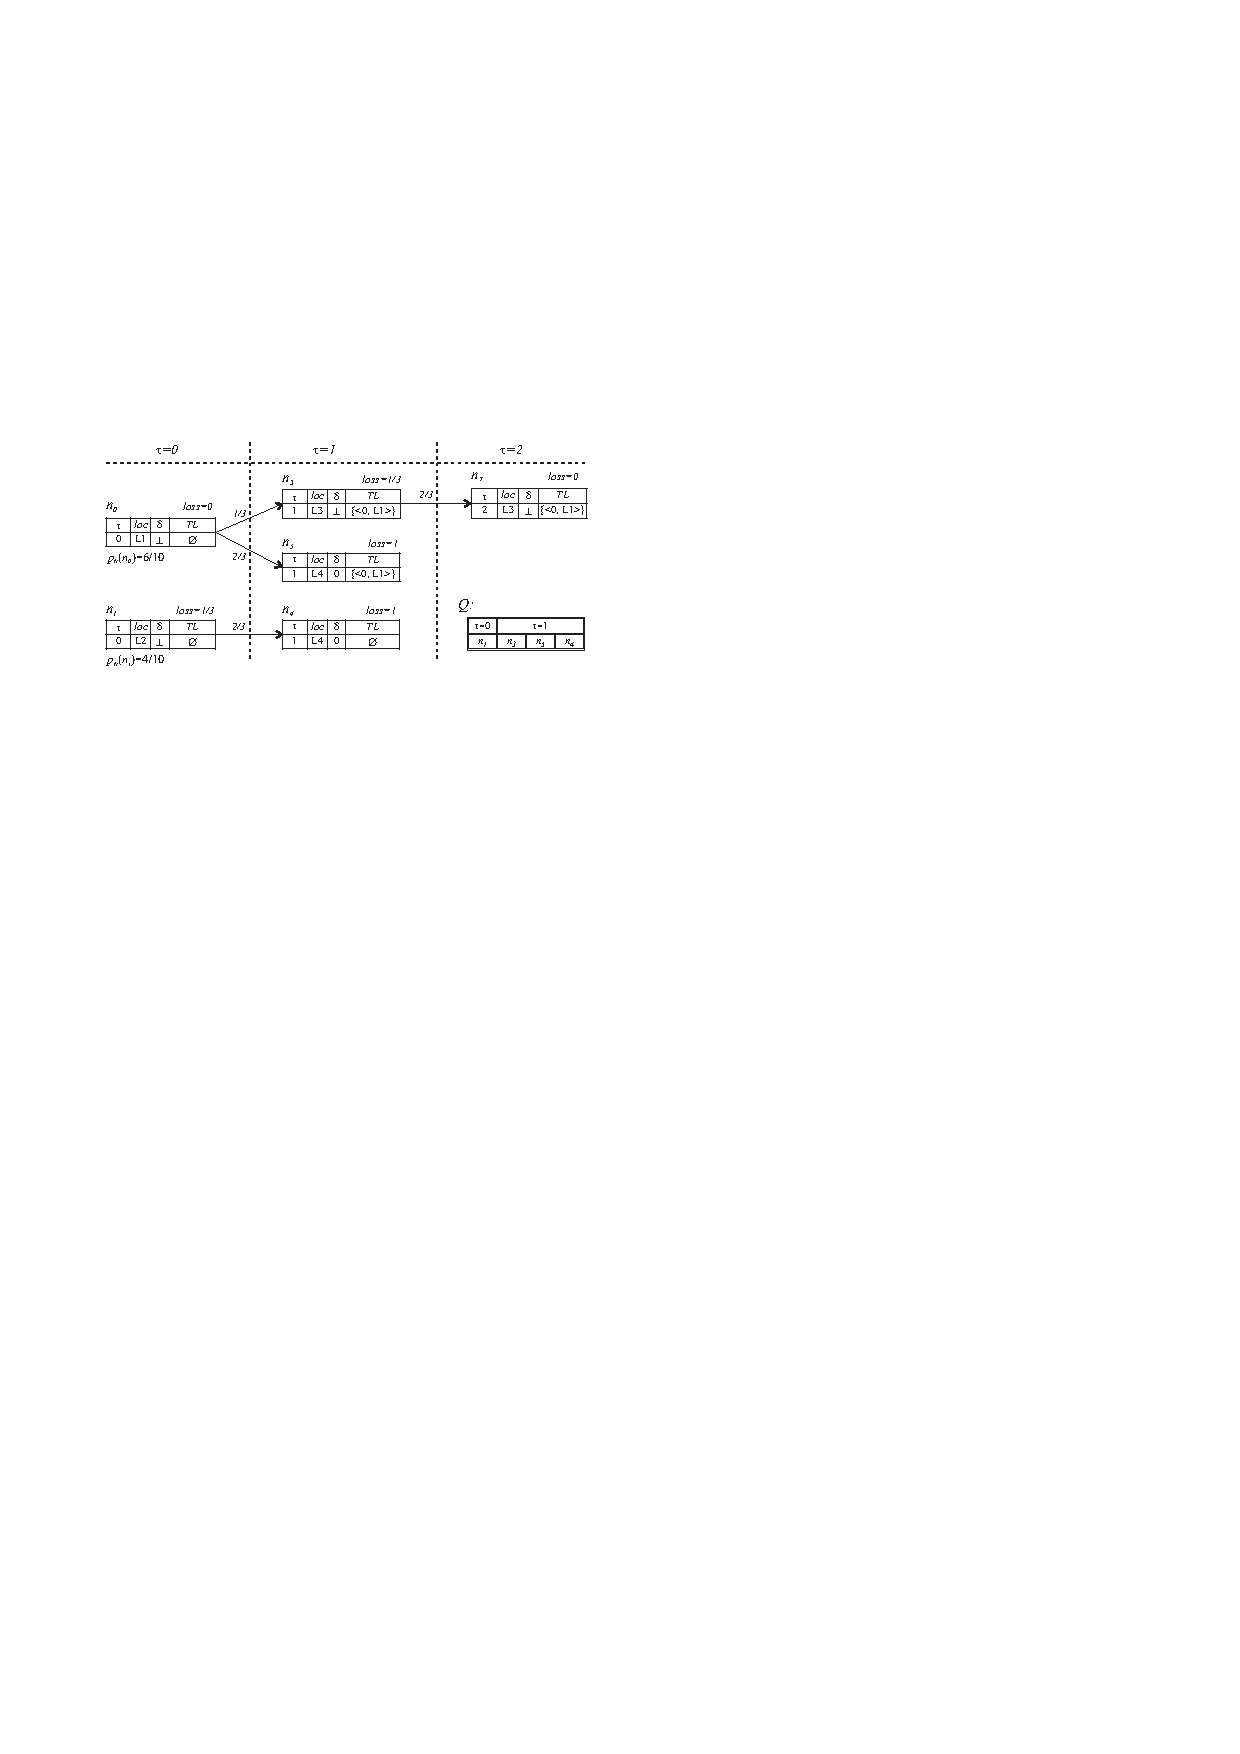
\includegraphics[width=0.5\columnwidth]{figures/3-4/3-4-7.pdf}
\end{figure}

\vspace{-15pt}

\begin{example}
  \ssize{
  At iteration $\tau = 1$, $n_3$, $n_5$ and $n_4$ are processed. In the case $n = n_3$, the inner loop only processes the location node $n_7$ where is the only successor of $n_3$. Thus, $n_7$ is added to $N$, the edge $\langle n_3,n_7 \rangle$ is added to $E$, and the probability $p(\langle n_3, n_7 \rangle) = p(\langle 2, L_3 \rangle) = 2/3$. Next, $n_3.loss$ is assigned with $1 - 2/3 = 1/3$ and $n_3$ is added to $Q$.\\
  In both the cases $n = n_5$ and $n = n_4$, since there is no location node which is a successor of $n_5$ or $n_4$, $n_5.loss$ and $n_4.loss$ are both assigned with 1 and both $n_5$ and $n_4$ are added to $Q$.
  }
\end{example}

\end{frame}

%------------------------------------------------

\begin{frame}
\frametitle{The Cleansing Algorithm: Backward Phase}

\begin{columns}

  \column{0.42\textwidth}
  \begin{figure}[tb]
    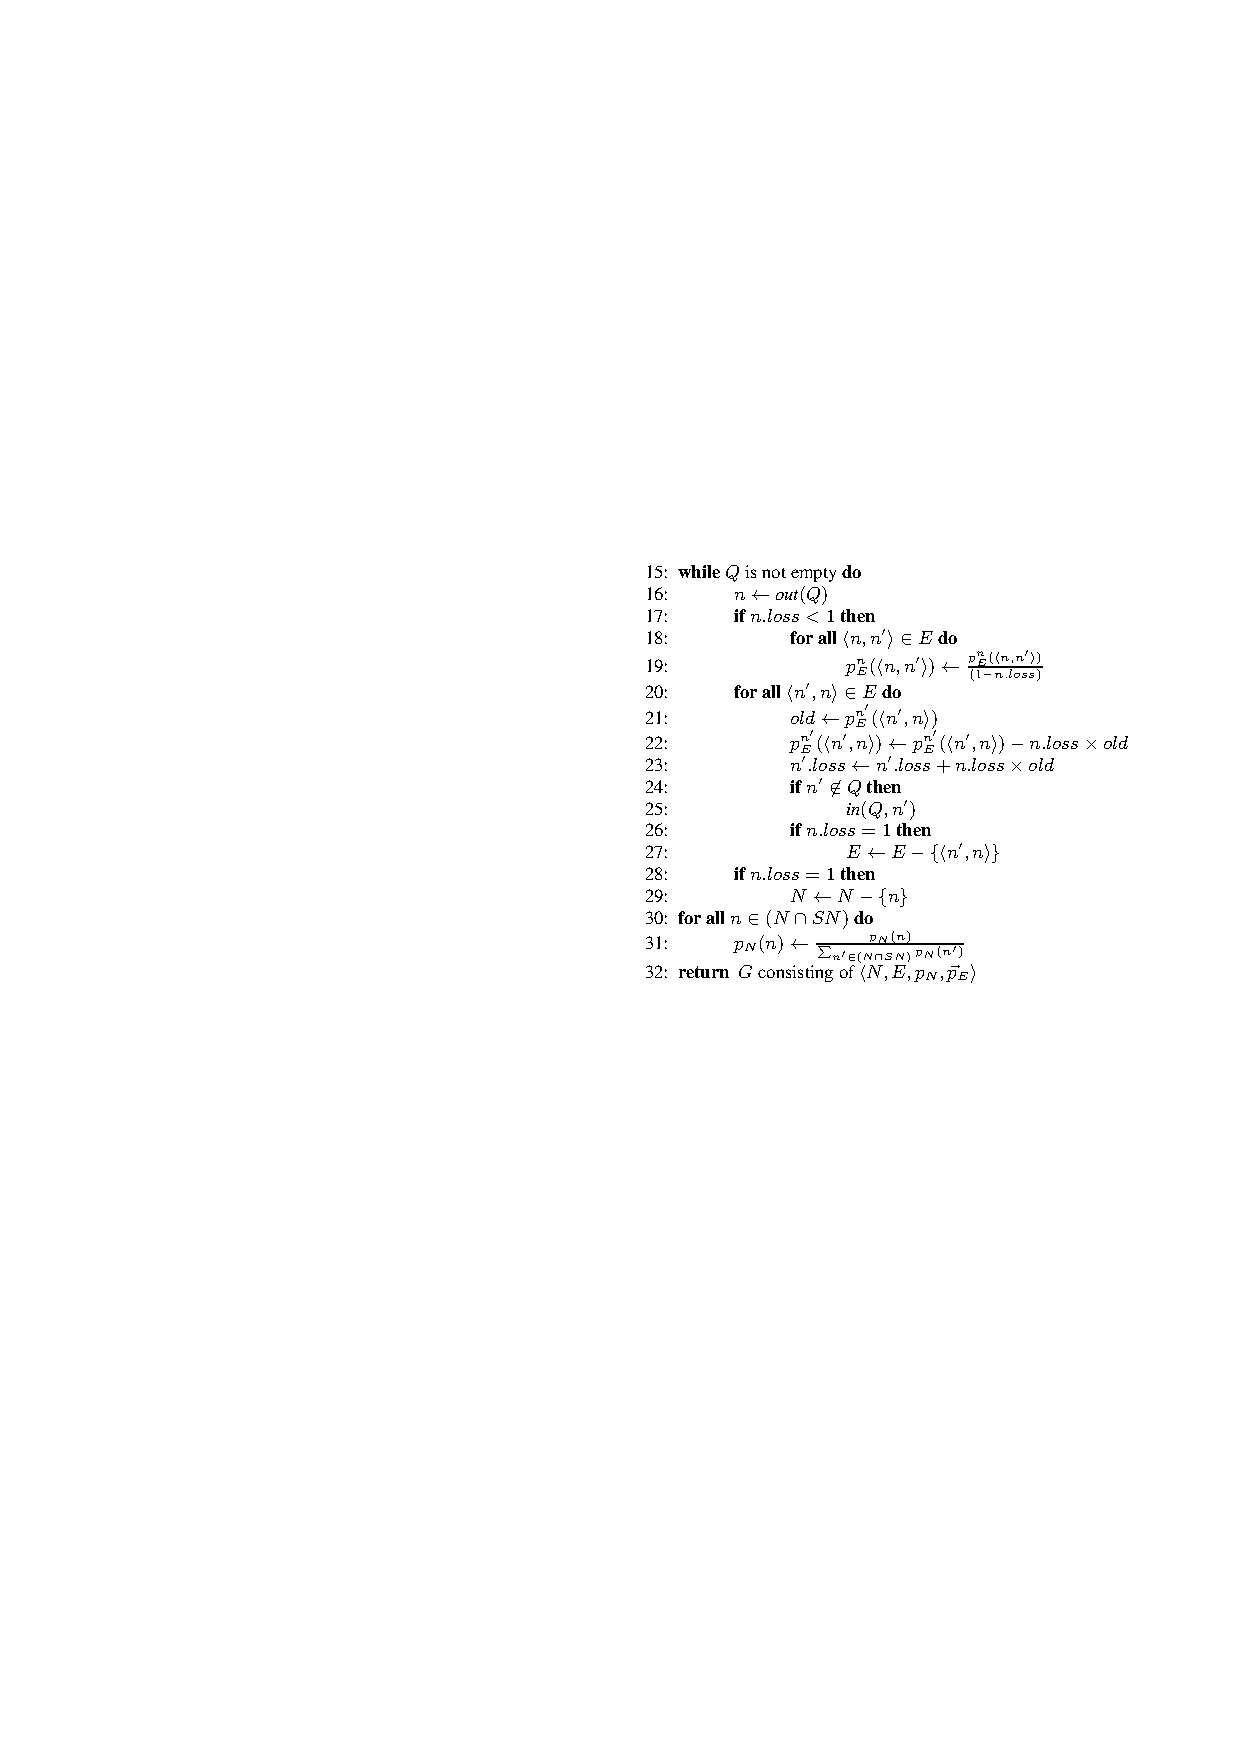
\includegraphics[width=\columnwidth]{figures/3-4/3-4-8.pdf}
  \end{figure}

  \column{0.58\textwidth}
  \begin{sitemize}
    \item line 16: a node $n$ among those having the highest timestamp is extracted from $Q$;
    \item line 19: if $n.loss$ is lower than 1 (meaning that $n$ has at least one outgoing edge), the probability of each of the outgoing edges of $n$ is conditioned, i.e., its current value is divided by the sum of the probabilities of the outgoing edges of $n$;
    \item line 22: the probability of each ingoing edge $\langle n',n \rangle$ of $n$ is decremented by the value of $n.loss$ multiplied by the old probability value of the edge $\langle n',n \rangle$;
    \item line 23: the value of $n'.loss$ of each node $n'$ of which $n$ is successor is incremented of the value of $n.loss$ multiplied by the old probability value of the edge $\langle n',n \rangle$;
  \end{sitemize}

\end{columns}

\end{frame}

%------------------------------------------------

\begin{frame}
\frametitle{The Cleansing Algorithm: Backward Phase}

\begin{columns}

  \column{0.42\textwidth}
  \begin{figure}[tb]
    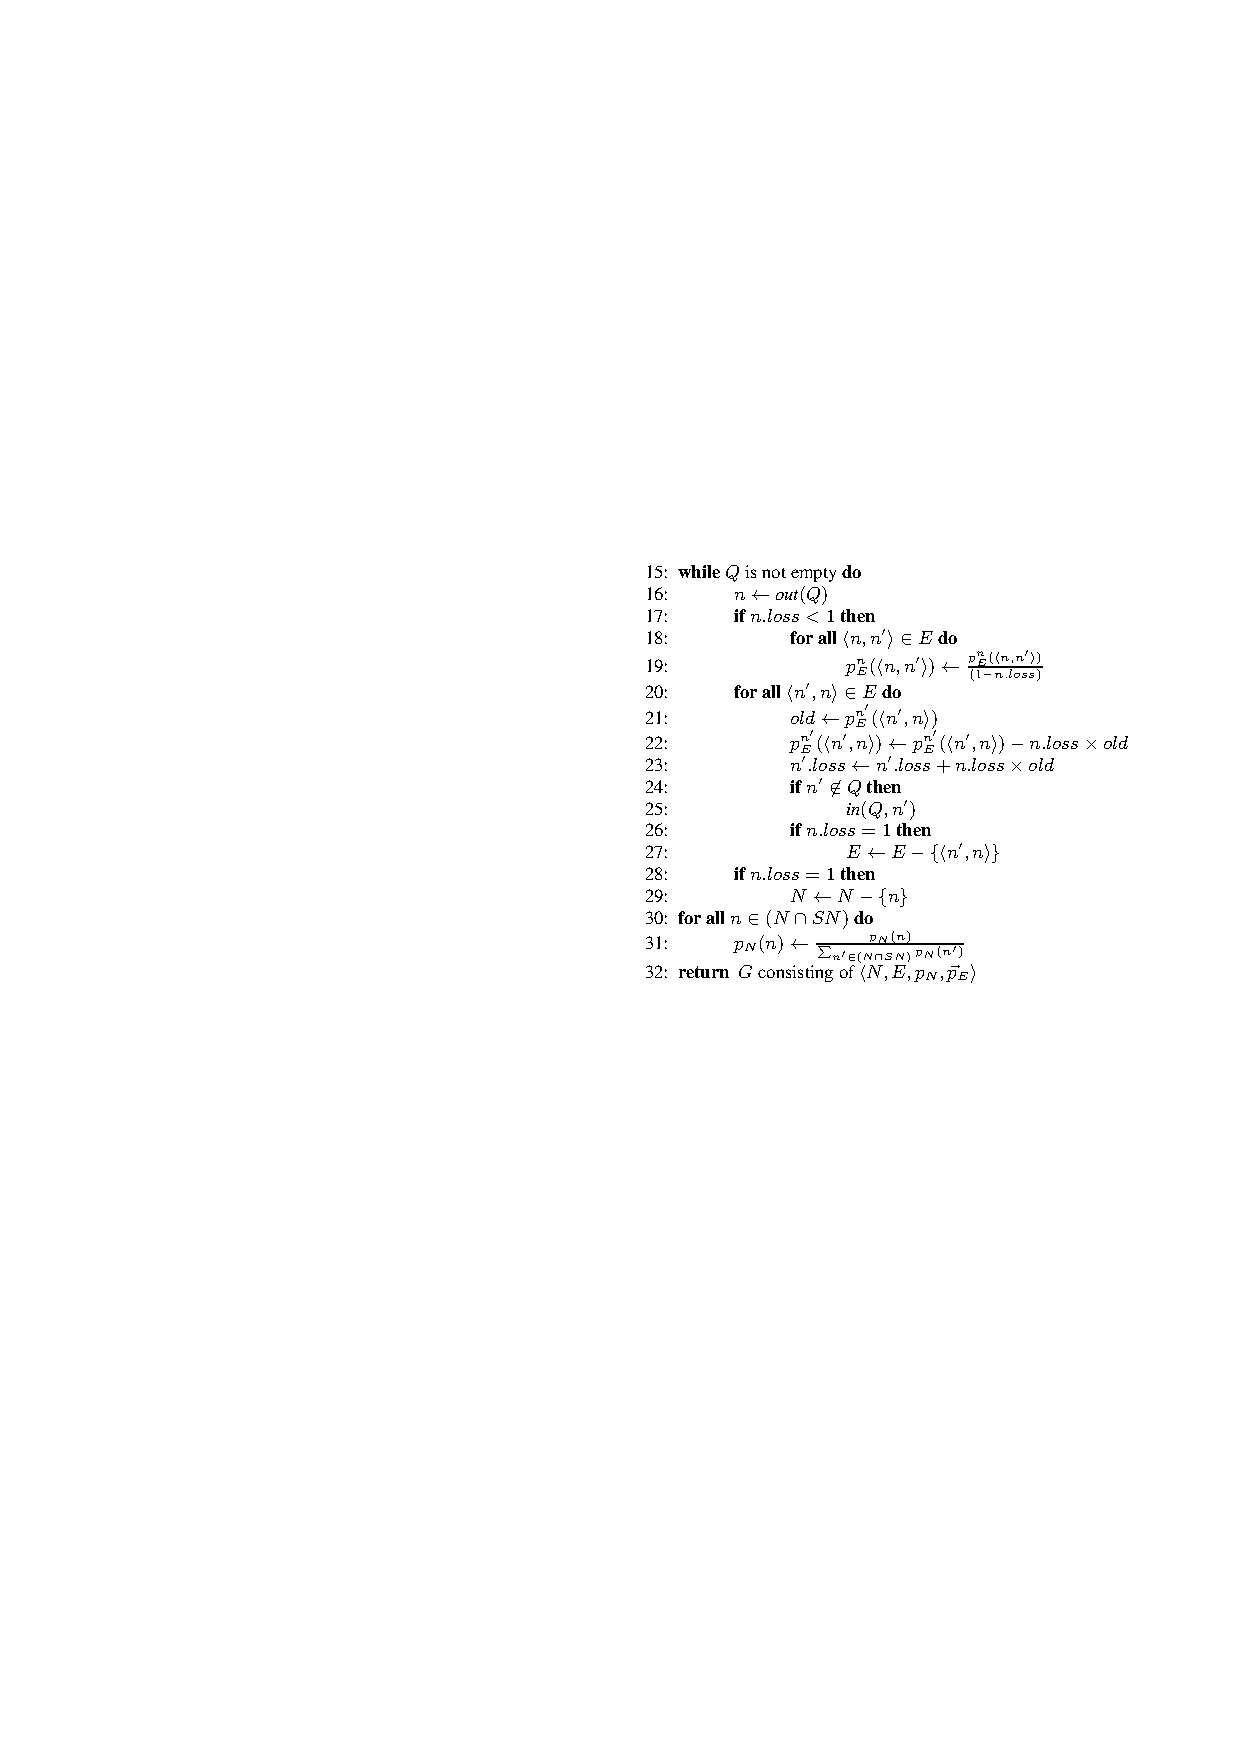
\includegraphics[width=\columnwidth]{figures/3-4/3-4-8.pdf}
  \end{figure}

  \column{0.58\textwidth}
  \begin{sitemize}
    \item line 25: since $n'.loss$ has been incremented and thus it is greater than 0, node $n'$ is added to $Q$ if it's not already present in it;
    \item line 27: furthermore, in the case $n.loss = 1$, the edge $\langle n',n \rangle$ is removed from $E$;
    \item line 29: at the end of the loop scanning the ingoing edges of $n$, if $n.loss = 1$, $n$ is removed from $N$;
    \item line 31: the probability $p_N(n)$ of each source node $n$ in $N$ is conditioned, i.e., $p_N(n)$ is divided by the sum of the probabilities of the source nodes belonging to $N$.
  \end{sitemize}

\end{columns}


\end{frame}

%------------------------------------------------

\begin{frame}
\frametitle{The Cleansing Algorithm: Backward Phase}

\begin{figure}[tb]
  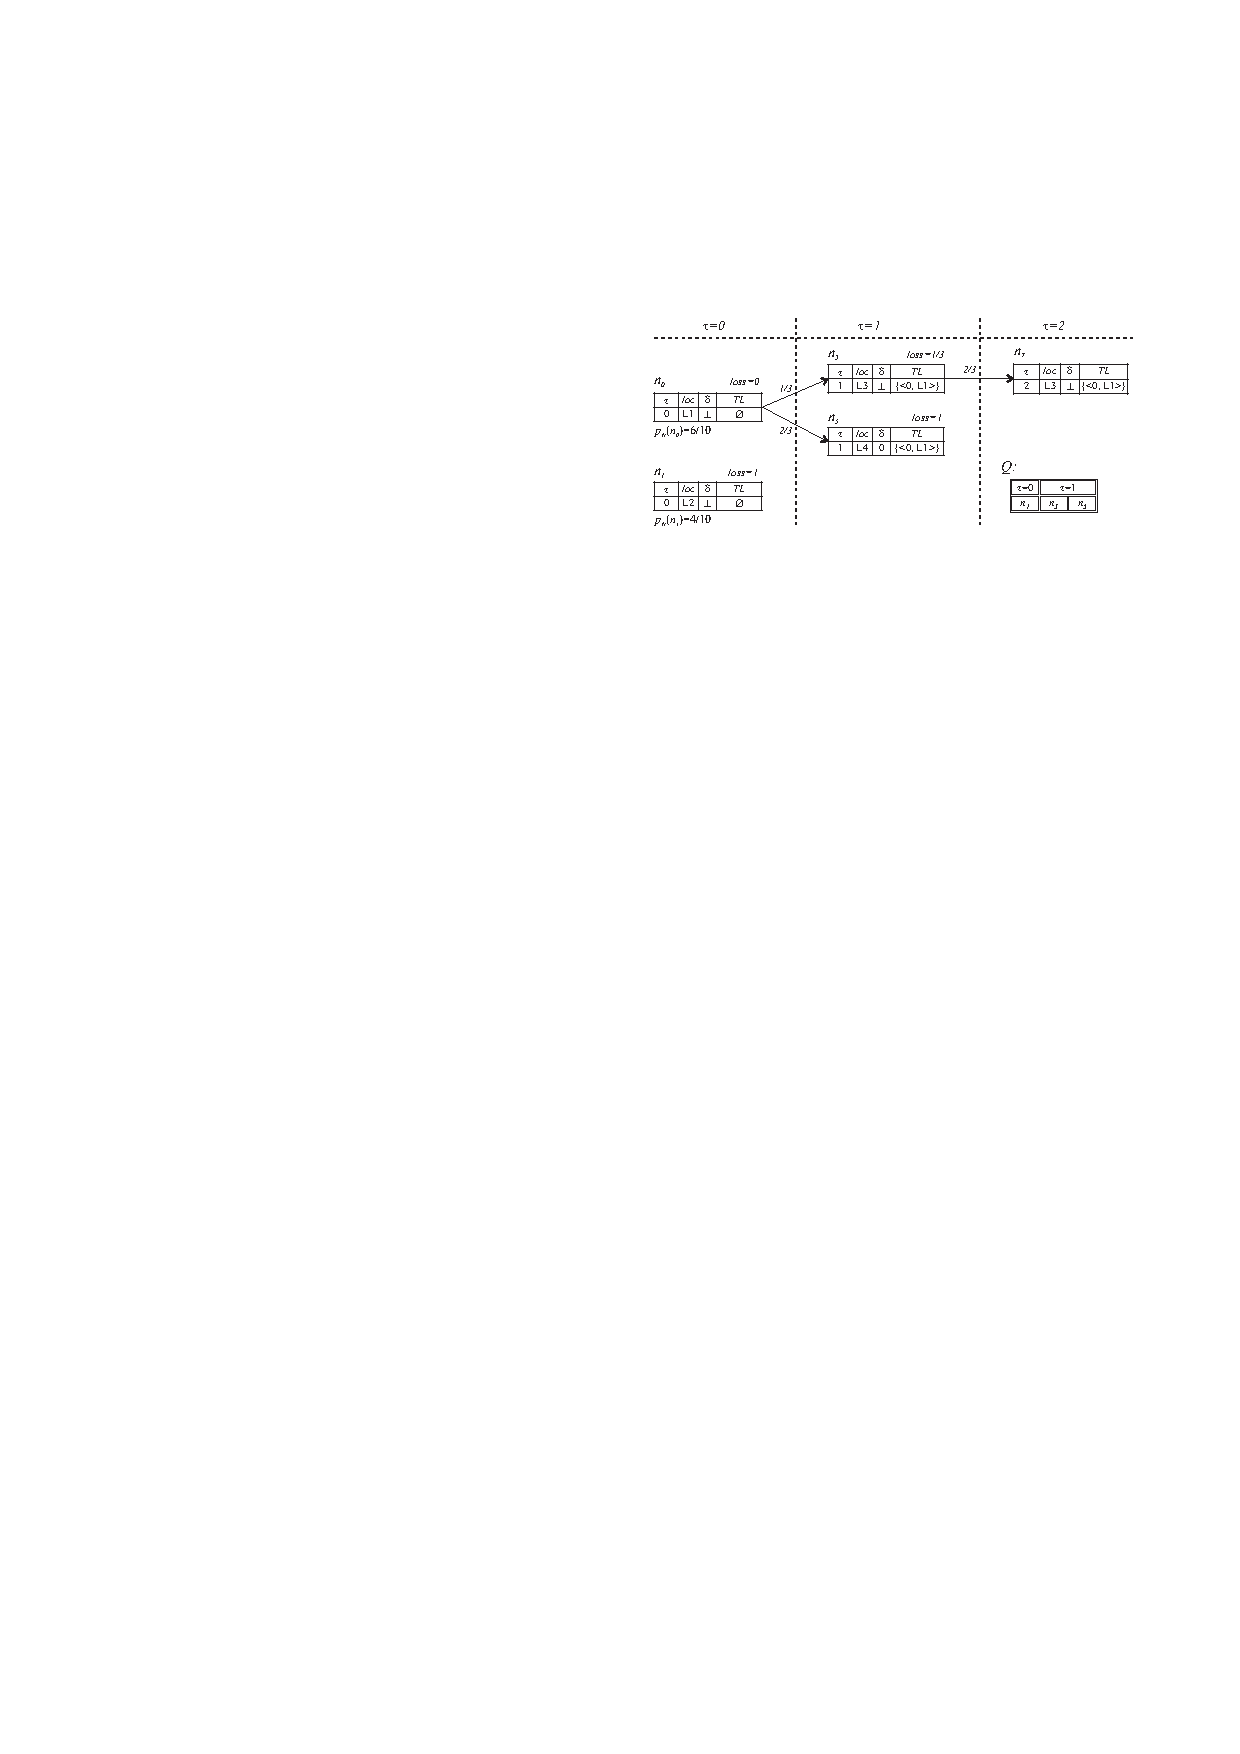
\includegraphics[width=0.5\columnwidth]{figures/3-4/3-4-9.pdf}
\end{figure}

\vspace{-15pt}

\begin{example}
  \ssize{
  At the first iteration of the while loop, node $n_4$ is removed from $Q$ since $n_4.loss$ is equal to 1. Thus, the algorithm processes the ingoing edges of $n_4$. Specifically, as $n_4$ has only the incoming edge $\langle n_1,n_4 \rangle$, the probability value of $\langle n_1,n_4 \rangle$ is set to $2/3 -2/3 = 0$, and, correspondingly variable $n_1.loss$ is set to $1/3 + 2/3 = 1$. Then the edge $\langle n_1,n_4 \rangle$ is removed from $N$.
  }
\end{example}

\end{frame}
